\documentclass[a4paper]{article}
\usepackage[normalem]{ulem}
\usepackage{graphicx}
\usepackage[font=small,labelfont=bf]{caption}

% impostazioni generali
%Tutti gli usepackage vanno qui
\usepackage[table]{xcolor}
\usepackage{geometry}
\usepackage[italian]{babel}
\usepackage[utf8]{inputenc}
\usepackage{tabularx}
\usepackage{longtable}
\usepackage{hyperref}
\usepackage{enumitem}
\usepackage{array} 
\usepackage{booktabs}
\newcolumntype{M}[1]{>{\centering\arraybackslash}m{#1}}
\usepackage[toc]{appendix}
\usepackage{caption}

\hypersetup{
	colorlinks=true,
	linkcolor=blue,
	filecolor=magenta,
	urlcolor=blue,
}
% Numerazione figure
\let\counterwithout\relax
\let\counterwithin\relax
\usepackage{chngcntr}

% distanziare elenco delle figure e delle tabelle
\usepackage{tocbasic}
\DeclareTOCStyleEntry[numwidth=3.5em]{tocline}{figure}% for figure entries
\DeclareTOCStyleEntry[numwidth=3.5em]{tocline}{table}% for table entries


%\counterwithout{table}{section}
%\counterwithout{figure}{section}
\captionsetup[table]{font=small,skip=5pt} 

\usepackage[bottom]{footmisc}
\usepackage{fancyhdr}
\setcounter{secnumdepth}{4}
\usepackage{amsmath, amssymb}
\usepackage{array}
\usepackage{graphicx}

\usepackage{ifthen}

\usepackage{float}
\restylefloat{table}

\usepackage{layouts}
\usepackage{url}
\usepackage{comment}
\usepackage{eurosym}

\usepackage{lastpage}
\usepackage{layouts}
\usepackage{eurosym}

\geometry{a4paper,top=3cm,bottom=4cm,left=2.5cm,right=2.5cm}

%Comandi di impaginazione uguale per tutti i documenti
\pagestyle{fancy}
\lhead{
\includegraphics[scale=0.25]{template/images/logo-inline.png}}

%Titolo del documento

%\rfoot{\thepage}
\cfoot{Pagina \thepage\ di \pageref{LastPage}}
\setlength{\headheight}{35pt}
\setcounter{tocdepth}{5}
\setcounter{secnumdepth}{5}
\renewcommand{\footrulewidth}{0.4pt}

% multirow per tabelle
\usepackage{multirow}

% Permette tabelle su più pagine
%\usepackage{longtable}


%COMANDI TABELLE
\newcommand{\rowcolorhead}{\rowcolor[HTML]{731733}}
\newcommand{\captionline}{\rowcolor[HTML]{FFFFFF}} %comando per le caption delle tabelle
\newcommand{\cellcolorhead}{\cellcolor[HTML]{007c95}}
\newcommand{\hlinetable}{\arrayrulecolor[HTML]{007c95}\hline}

%intestazione
% check for missing commands
\newcommand{\headertitle}[1]{\textbf{\color{white}#1}} %titolo colonna
\definecolor{pari}{HTML}{dcbac2}
\definecolor{dispari}{HTML}{f5f5f5}

% comandi \textit{Glossario}
\newcommand{\glo}{$_{G}$}
\newcommand{\glosp}{$_{G}$ }

%comando signature
\newcommand\signature[2]{% Name; Department
\noindent\begin{minipage}{5cm}
    \noindent\vspace{3cm}\par
    \noindent\rule{5cm}{1pt}\par
    \noindent\textbf{#1}\par
    \noindent#2%
\end{minipage}}


%label custom
\makeatletter
\newcommand{\uclabel}[2]{%
	\protected@write \@auxout {}{\string \newlabel {#1}{{#2}{\thepage}{#2}{#1}{}} }%
	\hypertarget{#1}{#2}
}
\makeatother

%riportare pezzi di codice
\definecolor{codegray}{gray}{0.9}
\newcommand{\code}[1]{\colorbox{codegray}{\texttt{#1}}}

% dati relativi alla prima pagina
\makeindex
\begin{document}
\counterwithin{table}{section}

% Prima pagina
\thispagestyle{empty}
\renewcommand{\arraystretch}{1.3}


\begin{titlepage}
	\begin{center}
		
	
\includegraphics[scale = 0.6]{template/images/logo-circle.png}
	\\[0.8cm]
	\href{mailto:6bitbusters@gmail.com}		      	
	{\large{\textit{6bitbusters@gmail.com} } }\\[0.8cm]
	
	\Huge \textbf{Norme di progetto} \\[0.5cm]

	% Informazioni sul documento
	\large \textbf{Informazioni sul documento} \\
	\rule{0.6\textwidth}{0.4pt}
	\\[0.5cm]
	\begin{tabular}{r|l}
		\textbf{Versione} & 1.0.0\\
		\textbf{Stato} & Approvato\\
		\textbf{Uso} & Interno\\                         
		\textbf{Approvazione} & Soranzo Andrea\\                      
		\textbf{Verifica} & Pincin Matteo\\ & Diviesti Filippo\\ & Bergamin Elia\\ & Djossa Edgar\\                        
		\textbf{Redazione} & Djossa Edgar \\ & Pincin Matteo \\ & Soranzo Andrea\\ & Chilese Elena \\ & Bergamin Elia\\
		\textbf{Distribuzione} & \textit{Six Bit Busters} \\ & Prof. Vardanega Tullio \\ & Prof. Cardin Riccardo
	\end{tabular}	
	\\[0.8cm]

 % Descrizione
	\large \textbf{Descrizione} \\
	Questo documento contiene le norme di progetto seguite dal gruppo \textit{Six Bit Busters}.
	
	
	
	\end{center}
\end{titlepage}


% Diario delle modifiche

\section*{Registro delle modifiche}

\newcommand{\changelogTable}[1]{

\renewcommand{\arraystretch}{1.5}
\rowcolors{2}{pari}{dispari}
\begin{longtable}{ %0.87
		>{\centering}M{0.10\textwidth} 
		>{\centering}M{0.11\textwidth}
		>{\centering}M{0.19\textwidth}
		>{\centering}M{0.28\textwidth} 
		>{\centering\arraybackslash}M{0.19\textwidth} 
		 }
	\rowcolorhead
	\headertitle{Versione} &
	\centering \headertitle{Data} &	
	\headertitle{Autore} &
	\headertitle{Descrizione} & 
	\headertitle{Verificatore} 
	\endfirsthead	
	\endhead
	
	#1

\end{longtable}
\vspace{-2em}

}


\changelogTable{
1.0.0& xxx & xxx & - &  Approvazione documento\tabularnewline
0.1.0& xxx & xxx & - &  Verifica documento\tabularnewline
0.0.3& xxx & xxx & - &  Stesura pro e contro\tabularnewline
	0.0.2& xxx & xxx & - &  Stesura introduzione\tabularnewline
	0.0.1 & 17-10-2024 & Chilese Elena & - &  Creazione struttura e template documento \\
}
\pagebreak

% Indice
{
    \hypersetup{linkcolor=black}
    \tableofcontents
}
\pagebreak

% Tabelle 
{
    \listoftables
}
\pagebreak

% Figure
{
    \listoffigures
}
\pagebreak

\section*{Introduzione}
\addcontentsline{toc}{section}{Introduzione}
p
    Il presente documento costituisce una raccolta di definizioni chiare e precise dei termini non
    comuni utilizzati nella documentazione prodotta dal gruppo. \\
    Negli altri documenti, i termini presenti nel \textit{Glossario} sono contrassegnati dalla lettera g a pedice (es. termine\textsubscript{g}).\\
    Per velocizzare la ricerca di un vocabolo, il \textit{Glossario} è suddiviso in sezioni,
    una per ogni lettera, contenente le parole che hanno come iniziale quella lettera. Le sezioni sono 
    naturalmente disposte in ordine alfabetico.\\
    Per evitare inconsistenze di forma, per i termini stranieri è indicato se sono sostantivi (s.) o aggettivi (agg.).
    Nei sostantivi è specificato se sono comuni (c.) o propri (p.), maschili (m.) o femminili (f.).\\
    Il \textit{Glossario} è redatto in maniera incrementale, in base all'utilizzo
    di nuovi termini da definire.

\pagebreak

\section{Analisi dei rischi}
In questa sezione sono riassunti i rischi che il gruppo potrebbe dover affrontare a seguito dell'aggiudicazione del capitolato \textit{3Dataviz}.
Il nostro obiettivo è adottare decisioni e scelte che permettano di gestire il progetto riducendo al minimo i problemi.
Tuttavia, nel caso in cui questi si verifichino, vogliamo essere preparati con soluzioni concrete e immediatamente adottabili.
\\I rischi sono stati suddivisi in quattro differenti categorie e, per ciascun rischio, dopo una breve descrizione, viene presentata l'analisi dei seguenti punti:
\begin{itemize}
    \item \textbf{Nome}: identifica il rischio;
    \item \textbf{Descrizione}: descrizione del rischio atteso;
    \item \textbf{Prob.} (Probabilità di occorrenza): indica la probabilità con cui è possibile si verifichi il rischio (Bassa=B, Media=M, Alta=A);
    \item \textbf{Per.} (Grado di pericolosità): indica il grado di pericolosità del rischio (Basso=B ,Medio=M, Alto=A);
    \item \textbf{Misure preventive}: indica le misure adottate per cercare di evitare il verificarsi del rischio;
    \item \textbf{P.Cont.} (Piano di Contingenza): indica come far fronte al rischio nel caso in cui esso si verifichi. 
\end{itemize}
\newcommand{\riskTable}[1]{
	 

\renewcommand{\arraystretch}{1.5}
\rowcolors{2}{pari}{dispari}
\begin{longtable}{ 
		>{\centering}M{0.2\textwidth} 
		>{\raggedright}M{0.33\textwidth} 
		>{\centering}M{0.05\textwidth}
		>{\centering}M{0.05\textwidth}
		>{\raggedright}M{0.24\textwidth} 
		 }
	\rowcolorhead
	\headertitle{Nome} &
	\headertitle{Descrizione} &
	\centering \headertitle{Prob.} &	
	\headertitle{Per.} &
	\headertitle{Misure preventive}
	\endfirsthead	
	\endhead
	
	#1

\end{longtable}
\vspace{0.2em}

}

\subsection{Rischi riguardanti i requisiti}
\riskTable{
    \textbf{Analisi dei requisiti} & Richiede un impegno significativo da parte del gruppo ed è fondamentale per capire cosa dovrà fare il prodotto. Il rischio principale è tralasciare aspetti importanti, causando discrepanze tra gli impegni preventivati e quelli effettivi.
     & M & A & Analizzare in dettaglio tutti i casi d’uso e i relativi requisiti, mantenendo un dialogo aperto e costante con il proponente.\tabularnewline
     \multicolumn{5}{l}{\textbf{P.Cont.:} Organizzare colloqui con il proponente per discutere sul da farsi.}\tabularnewline
     \textbf{Cambiamento dei requisiti iniziali} & I requisiti iniziali potrebbero subire modifiche e/o aggiunte da parte del proponente.
     & M & M & Realizzare un'analisi dei requisiti il più possibile chiara e precisa.\tabularnewline
     \multicolumn{5}{l}{\textbf{P.Cont.:} Discutere e comprendere appieno ogni cambiamento insieme al proponente.}\tabularnewline
     \captionline\caption{Rischi riguardanti i requisiti}
}
\pagebreak
\subsection{Rischi tecnologici}
\riskTable{
    \textbf{Strumenti e tecnologie sconosciute} & Il progetto richiede l'utilizzo di software per la creazione di grafici 3D, oltre a librerie JavaScript e Framework a noi attualmente poco conosciuti.
     & A & M & Valutare ogni strumento o tecnologia ed esercitarsi per scegliere quello più adatto. Sfruttare le conoscenze pregresse per facilitare la divisione del lavoro e per non concentrarsi troppo su funzionalità meno rilevanti.\tabularnewline
     \multicolumn{5}{p{\dimexpr\textwidth-2\tabcolsep\relax}}{\textbf{P.Cont.:} Se l’utilizzo di uno strumento o di una tecnologia causa ritardi, si procederà con una maggiore suddivisione più efficiente del lavoro e, in casi estremi, si valuterà un’alternativa, sempre confrontando il proponente.}\tabularnewline
     \textbf{Problemi hardware o software} & Problemi causati da PC malfunzionanti e problemi software derivati da guasti.
     & M & B & Condivisione dei file di progetto in un repository comune utilizzando un sistema di versionamento distribuito atto a garantire una gestione collaborativa delle modifiche.\tabularnewline
     \multicolumn{5}{p{\dimexpr\textwidth-2\tabcolsep\relax}}{\textbf{P.Cont.:} Utilizzare dispositivi secondari per continuare il lavoro.}\tabularnewline
     \captionline\caption{Rischi tecnologici}
}

\subsection{Rischi organizzativi}
\riskTable{
    \textbf{Pianificazione inadeguata} & La pianificazione di un intero progetto di questa portata include una corretta individuazione delle attività da svolgere e un'adeguata suddivisione dei compiti. Tuttavia, l'inesperienza dei membri del gruppo può provocare ritardi e spreco di risorse.
     & A & A & Pianificazione su brevi periodi di tempo e con una visione pessimistica.\tabularnewline
     \multicolumn{5}{l}{\textbf{P.Cont.:} Stilare un nuovo piano di lavoro che ottimizzi le risorse e la suddivisione del lavoro.}\tabularnewline
     \textbf{Distribuzione del lavoro} & La cattiva distribuzione del lavoro può causare un sovraccarico per un membro del gruppo, come altresì l'inattività di un membro.
     & M & M & Organizzare il lavoro tenendo conto delle disponibilità e delle capacità di ogni membro.\tabularnewline
     \multicolumn{5}{l}{\textbf{P.Cont.:} Suddivisione del lavoro in maniera più distribuita e uniforme.}\tabularnewline
     \captionline\caption{Rischi organizzativi}
}

\subsection{Rischi personali}
\riskTable{
    \textbf{Disponibilità dei componenti} & Il gruppo è composto da alcuni studenti-lavoratori i cui impegni non sono sempre conciliabili. Inoltre, ogni membro del gruppo è impegnato in altri esami universitari che possono richiedere una quantità significativa di tempo, soprattutto in prossimità della sessione invernale.
     & A & B & Organizzare con anticipo ogni incontro. Prevedere delle settimane di lavoro più intense ed altre meno, soprattutto in concomitanza con gli impegni sopra descritti.\tabularnewline
     \multicolumn{5}{p{\dimexpr\textwidth-2\tabcolsep\relax}}{\textbf{P.Cont.:} Il membro assente deve aggiornarsi sulle decisioni prese e acquisire le informazioni sui progressi in tempi brevi, così da riallinearsi rapidamente con il gruppo. Se l'assenza di uno o più membri causa ritardi significativi, il responsabile dovrà rivedere e ri-pianificare la suddivisione del lavoro.}\tabularnewline
     \textbf{Difficoltà comunicative} & La maggior parte degli incontri si svolgerà in modalità telematica.
     & B & M & Utilizzo di diversi strumenti di comunicazione.\tabularnewline
     \multicolumn{5}{p{\dimexpr\textwidth-2\tabcolsep\relax}}{\textbf{P.Cont.:} Ritrovo in presenza alla fine dell'ora di lezione o in un giorno preventivamente accordato.}\tabularnewline
     \textbf{Mancanza di esperienza personale} & Il progetto richiede l'acquisizione di competenze nuove per ogni membro del gruppo.
     & A & M & Iniziare a capire il funzionamento e sperimentare i nuovi strumenti e tecnologie da utilizzare.\tabularnewline
     \multicolumn{5}{p{\dimexpr\textwidth-2\tabcolsep\relax}}{\textbf{P.Cont.:} Se un membro riscontra parecchie difficoltà, può chiedere supporto agli altri membri e soprattutto al responsabile, il quale avrà il compito di trovare un compromesso atto a risolvere la situazione.}\tabularnewline
     \textbf{Conflitti interni} & I gruppi sono stati formati casualmente e i membri, non conoscendosi tra loro, potrebbero avere idee contrastanti.
     & B & M & Ciascun membro espone educatamente la propria idea, il responsabile sorveglierà ed agirà se necessario.\tabularnewline
     \multicolumn{5}{p{\dimexpr\textwidth-2\tabcolsep\relax}}{\textbf{P.Cont.:} Ogni decisione viene discussa e successivamente approvata a maggioranza.}\tabularnewline
     \captionline\caption{Rischi personali}
}

\pagebreak

\section{Modello di sviluppo}
\subsection{Modello agile}
Il gruppo \textit{Six Bit Busters} ha deciso di adottare un approccio ispirato
ai modelli agili, cercando di avvicinarsi il più possibile alle metodologie
tipiche del framework \textbf{Scrum}. Questa scelta è motivata dalle seguenti
considerazioni:
\begin{itemize}
    \item Scrum promuove la \textbf{collaborazione} continua tra i membri del team e gli
          stakeholder;
    \item Grazie agli sprint brevi, Scrum consente di \textbf{adattarsi} rapidamente a
          nuove esigenze o priorità;
    \item Gli sprint brevi consentono di individuare e \textbf{risolvere i problemi} più
          velocemente;
    \item Ad ogni sprint, il team si concentra su un \textbf{numero limitato di
              attività}, aumentando l'efficienza;
    \item I membri del team decidono come svolgere il lavoro durante gli sprint,
          aumentando il senso di \textbf{responsabilità};
    \item La natura iterativa di Scrum aiuta a suddividere grandi obiettivi in attività
          più \textbf{piccole e realizzabili}.
\end{itemize}

\subsection{Ruoli Scrum}
Scrum prevede tre ruoli (anche detti "responsabilità") che garantiscono che
ogni aspetto del lavoro condiviso sia gestito in modo efficace:
\begin{itemize}
    \item \textbf{Sviluppatori}: lavorano insieme per creare qualsiasi
          aspetto del prodotto. Le persone con qualsiasi competenza necessaria
          per creare il prodotto assumono la responsabilità di sviluppatore. Nel
          progetto didattico, tutti i membri del team ricoprono tale ruolo;
    \item \textbf{Product owner}: sviluppa e comunica l'obiettivo del prodotto
          ed è responsabile del product back-log. % trattino per andare a capo bene% 
          Conosce e comprende il dominio e il
          mercato del prodotto e vuole fornire agli utenti ciò di cui hanno bisogno.
          Nel progetto didattico, il product owner è il proponente;
    \item \textbf{Scrum master}: guida e dirige il team nell'adozione e
          nella pratica di Scrum. In particolare, cerca di massimizzare l'utilità
          degli eventi e degli artefatti. Nel progetto didattico, lo Scrum master è
          il membro del team con il ruolo di responsabile.
\end{itemize}

\subsection{Eventi Scrum}
Gli eventi Scrum sono preziose opportunità per ispezionare e adattare il
prodotto o il modo in cui il team lavora insieme.
\begin{itemize}
    \item \textbf{Sprint}: è un breve periodo di tempo in cui il team collabora per
          completare una determinata quantità di lavoro. Lo sprint contiene tutti gli altri eventi.
          Per il gruppo \textit{Six Bit Busters} ogni sprint dura due settimane;
    \item \textbf{Sprint planning}: stabilisce l'obiettivo dello sprint.
          Gli sviluppatori prevedono quali lavori ritengono di poter realizzare durante
          lo sprint per raggiungere l'obiettivo e come verrà completato il lavoro scelto.
          In base all'obiettivo viene creato un piano iniziale;
    \item \textbf{Daily scrum}: incontro giornaliero a cui partecipano tutti i membri del team,
          in cui ciascuno risponde alle seguenti domande:
          \begin{itemize}
              \item Cosa hai fatto ieri?
              \item Cosa farai oggi?
              \item C'è qualcosa che ti impedisce di farlo?
          \end{itemize}
          Ogni giorno lavorativo, al mattino, si svolge il daily scrum su un gruppo Telegram dedicato;
    \item \textbf{Sprint review}: il team esamina l'esito dello sprint con il
          product owner, che fornisce feedback su ciò che il team ha realizzato
          e sulla futura direzione dello sviluppo del prodotto. Il product backlog
          viene adattato in base a queste conversazioni;
    \item \textbf{Sprint retrospective}: è l'opportunità per il team di analizzare le
          proprie interazioni, collaborazioni, processi, strumenti e qualsiasi altro fattore
          ritenuto rilevante per la propria capacità di migliorare continuamente.
\end{itemize}

\subsection{Artefatti Scrum}
\begin{itemize}
    \item \textbf{Product backlog}: elenco ordinato o classificato di tutto ciò che potrebbe
          essere necessario per migliorare il prodotto, insieme all'obiettivo del prodotto;
    \item \textbf{Sprint backlog}: è composto dall'obiettivo dello sprint e dal set di
          elementi del product backlog che il product owner e gli sviluppatori hanno previsto
          di poter completare durante lo sprint corrente;
    \item \textbf{Incremento}: elemento del backlog completato in modo da fornire valore
          ed essere utilizzabile.
\end{itemize}
\subsection{Principi fondamentali}
\begin{itemize}
    \item \textbf{Trasparenza}: per prendere decisioni efficaci è necessario
          che il processo e i progressi del prodotto siano trasparenti,
          per garantire che tutti capiscano cosa stanno vedendo;
    \item \textbf{Ispezione}: le ispezioni regolari dei lavori in corso sono
          essenziali per mantenere il processo previsto e ottenere il risultato desiderato;
    \item \textbf{Adattamento}: consiste nell'esecuzione di tempestivi aggiustamenti
          al processo o al prodotto ogni volta che si verificano delle deviazioni. Ciò si
          realizza adattando il product backlog, il prodotto e i piani futuri a ogni sprint.\\\\
\end{itemize}

\begin{figure}[h!]
    \centering
    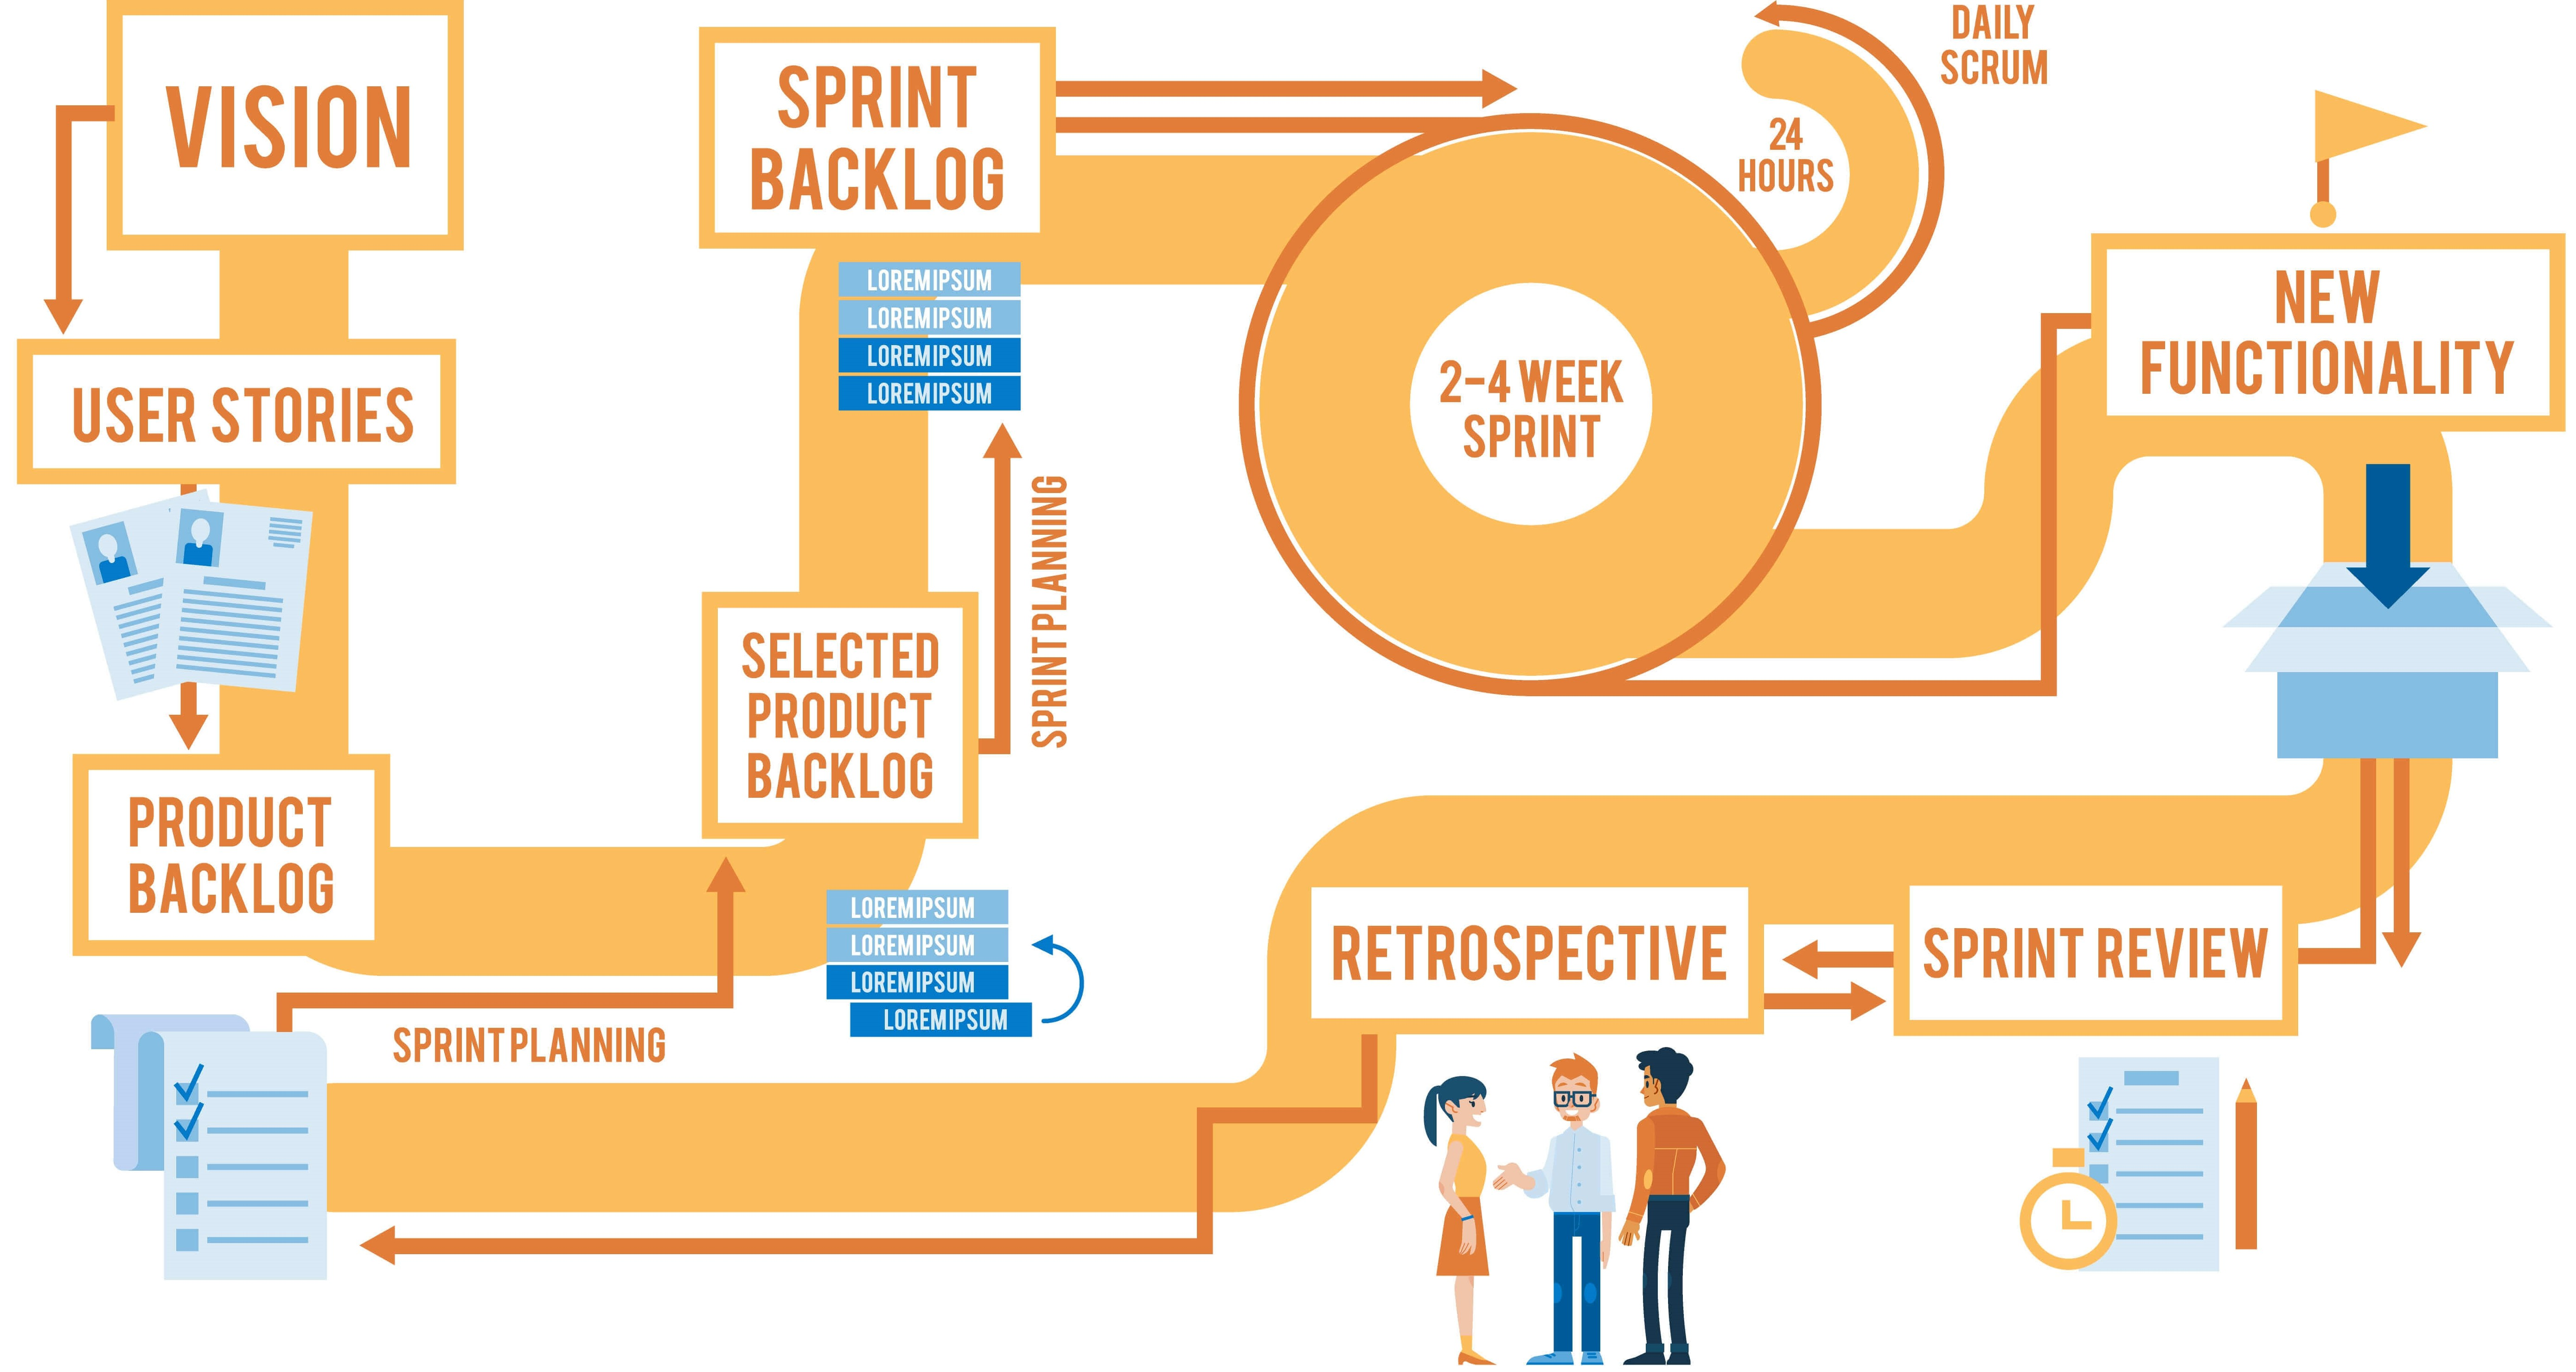
\includegraphics[scale = 0.08]{template/images/scrum.jpg}
    \caption{Il framework Scrum}
    \label{fig:2.1} % Etichetta per il riferimento
\end{figure}
\pagebreak

\section{Pianificazione}
Lo sviluppo del progetto è suddiviso nelle seguenti fasi:
\begin{itemize}
    \item RTB;
    \item PB.
\end{itemize}
\subsection{RTB}
Nel periodo dal 04/11/2024 al 17/01/2025 verranno prodotti i seguenti
documenti:
\begin{itemize}
    \item \textit{Norme di progetto};
    \item \textit{Piano di progetto};
    \item \textit{Analisi dei requisiti};
    \item \textit{Piano di qualifica};
    \item \textit{Glossario}.
\end{itemize}
Inoltre verrà realizzato il Proof of Concept (PoC), per valutare la fattibilità tecnologica del progetto.
\subsubsection{Sprint 1 (dal 11/11/2024 al 22/11/2024)}
In questo periodo verrà definito il way of working, documentato nelle
\textit{Norme di progetto}. Per quanto riguarda la gestione di progetto,
verranno pianificate le attività, stilato un preventivo e analizzati i rischi
che potrebbero incidere sullo svolgimento del progetto. Infine, si inizierà a
redigere il \textit{Glossario}, essenziale per garantire una comunicazione
chiara all'interno del team e con il proponente. \\
\begin{figure}[h!]
    \centering
    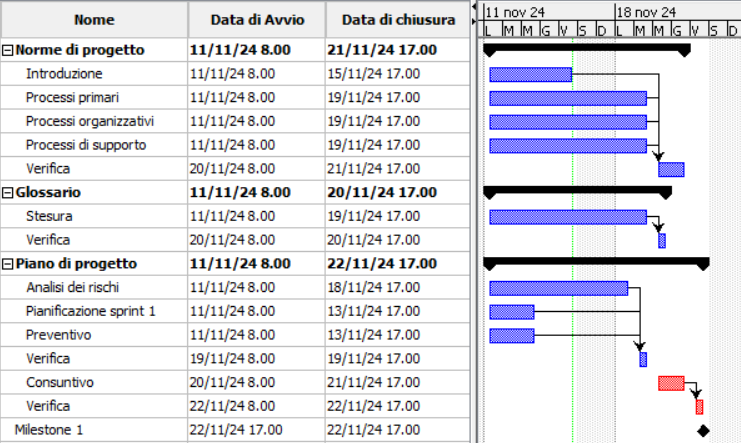
\includegraphics[scale = 0.85]{template/images/gantt1.png}
    \caption{Diagramma di Gantt sprint 1}
    \label{fig:3.1} % Etichetta per il riferimento
\end{figure}
\newpage

\subsubsection{Sprint 2 (dal 25/11/2024 al 06/12/2024)}
Durante questo secondo sprint, ci dedicheremo alla raccolta e all'analisi dei
requisiti, identificando i casi d'uso. Questi saranno documentati nel file
\textit{Analisi dei requisiti} per garantire una visione chiara degli obiettivi
del progetto. Continueremo l'espansione del \textit{Glossario}. Procederemo
inoltre con l'aggiornamento delle \textit{Norme di progetto} per assicurare una
gestione ottimale delle attività e delle risorse. Infine, con priorità minore,
inizieremo la stesura del \textit{Piano di qualifica}, necessario per definire
le metriche e le modalità di verifica della qualità del prodotto.

\begin{figure}[h!]
    \centering
    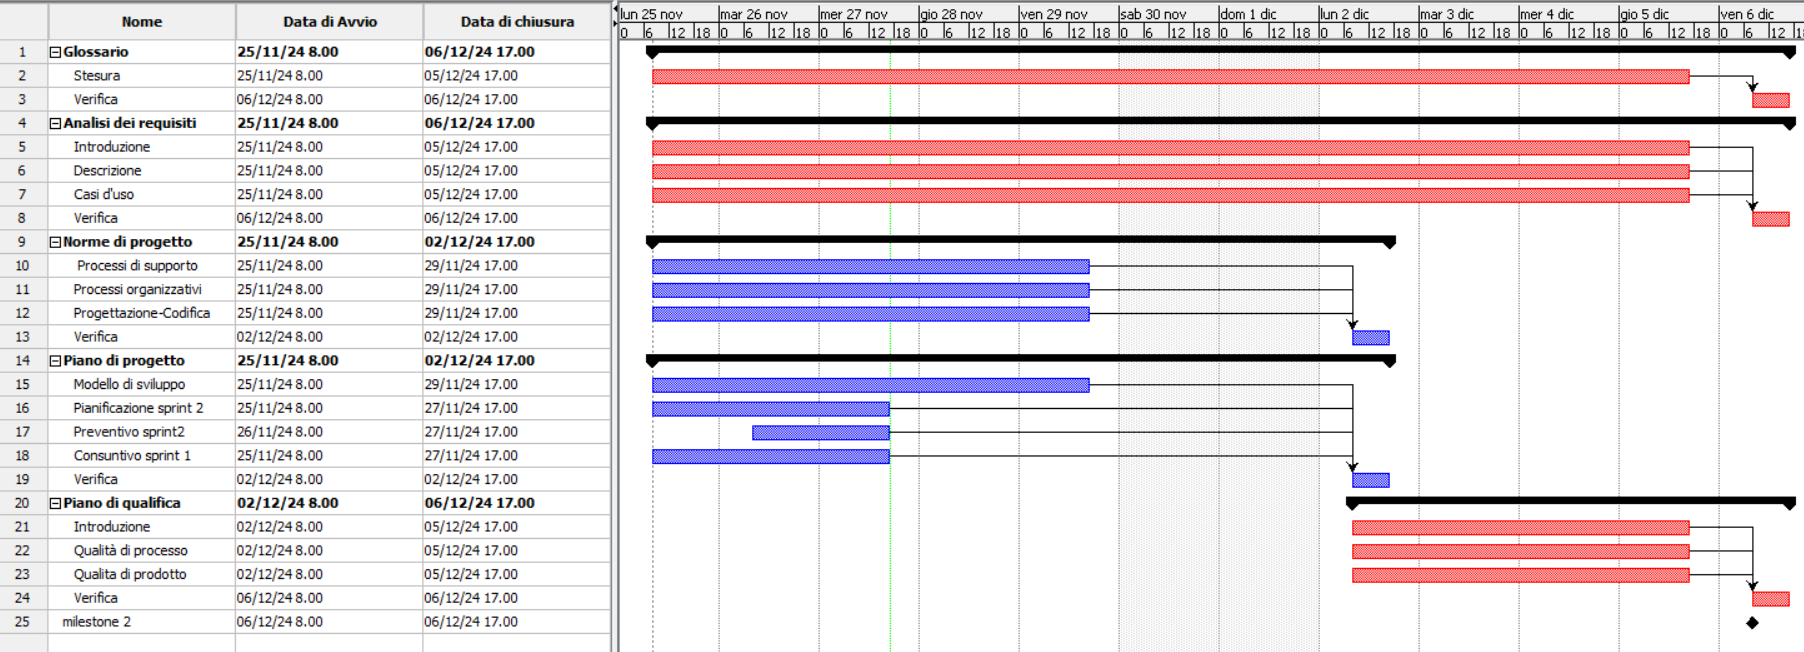
\includegraphics[scale = 0.3]{template/images/gantt2.png}
    \caption{Diagramma di Gantt sprint 2}
    \label{fig:3.2} % Etichetta per il riferimento
\end{figure}

\subsubsection{Sprint 3 (dal 09/12/2024 al 20/12/2024)}
In questo terzo sprint continueremo l'aggiornamento delle \textit{Norme di
    progetto} migliorando le regole che il team si pone di rispettare per garantire
un metodo di sviluppo efficace ed efficiente. E' prevista inoltre la stesura
delle metriche relative alla qualità del progetto e alla qualità del prodotto
nel \textit{Piano di qualifica}. Successivamente, in quanto di minore
importanza, è prevista la stesura della specifica dei test nel medesimo
documento. Per quanto riguarda l'\textit{Analisi dei requisiti} è pianificata
la stesura dei requisiti funzionali e di qualità ed eventualmente, a seguito di
un consulto con il proponente, si procederà anche con la stesura dei requisiti
di vincolo e prestazionali. Infine è prevista l'espansione del
\textit{Glossario}.

\begin{figure}[h!]
    \centering
    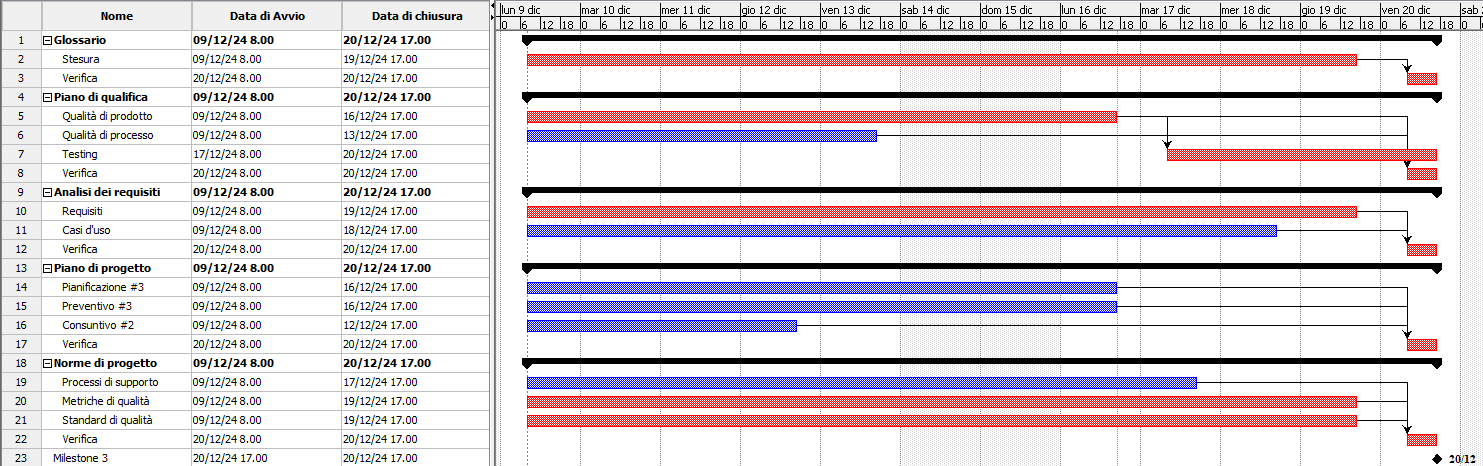
\includegraphics[scale = 0.3]{template/images/gantt3.png}
    \caption{Diagramma di Gantt sprint 3}
    \label{fig:3.3} % Etichetta per il riferimento
\end{figure}
\newpage

\subsubsection{Sprint 4 (dal 23/12/2024 al 10/01/2025)}
Durante questo quarto sprint (di durata maggiore a causa delle festività
natalizie), ci dedicheremo alla sistemazione dei casi d'uso, con l'obiettivo di
garantire che siano coerenti, completi e allineati ai requisiti del progetto.
Una delle attività di maggiore importanza sarà la realizzazione del Proof of
Concept (PoC). Esso servirà a validare le scelte tecniche adottate e a
dimostrare la fattibilità delle soluzioni individuate. Parallelamente, si
cercherà una soluzione per implementare in automatico il controllo della
qualità della documentazione prodotta tramite Indice Gulpease. Infine,
proseguiremo con l'espansione del \textit{Glossario}.

\begin{figure}[h!]
    \centering
    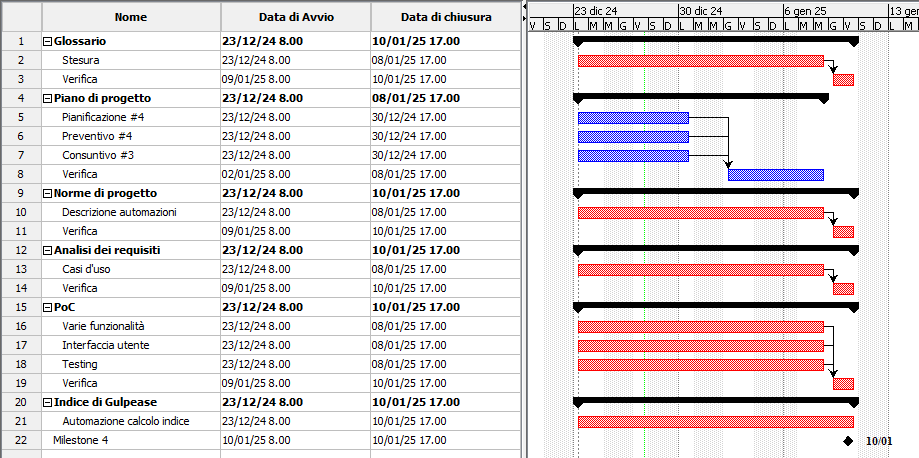
\includegraphics[scale = 0.45]{template/images/gantt4.png}
    \caption{Diagramma di Gantt sprint 4}
    \label{fig:3.4} % Etichetta per il riferimento
\end{figure}

\subsubsection{Sprint 5 (dal 13/01/2025 al 24/01/2025)}
In questo quinto sprint completeremo i documenti necessari per la RTB. Ci
concentreremo sul miglioramento dei documenti con un Indice Gulpease basso.
Vogliamo assicurarci che tutti superino la soglia minima richiesta. Inoltre,
aggiungeremo le sezioni mancanti nelle \textit{Norme di progetto}. Questo
renderà il documento più completo e facile da seguire. Rivedremo anche
l'\textit{Analisi dei requisiti} per migliorarne la chiarezza. Aggiorneremo i
casi d'uso e correggeremo i diagrammi UML per allinearli agli obiettivi del
progetto. Il \textit{Glossario} sarà ampliato con nuovi termini. Questo aiuterà
a rendere il progetto più accessibile. Infine, lavoreremo sul Proof of Concept
(PoC). Risolveremo gli ultimi bug grafici. L'obiettivo è presentare una
versione stabile, chiara e completamente funzionante.

\begin{figure}[h!]
    \centering
    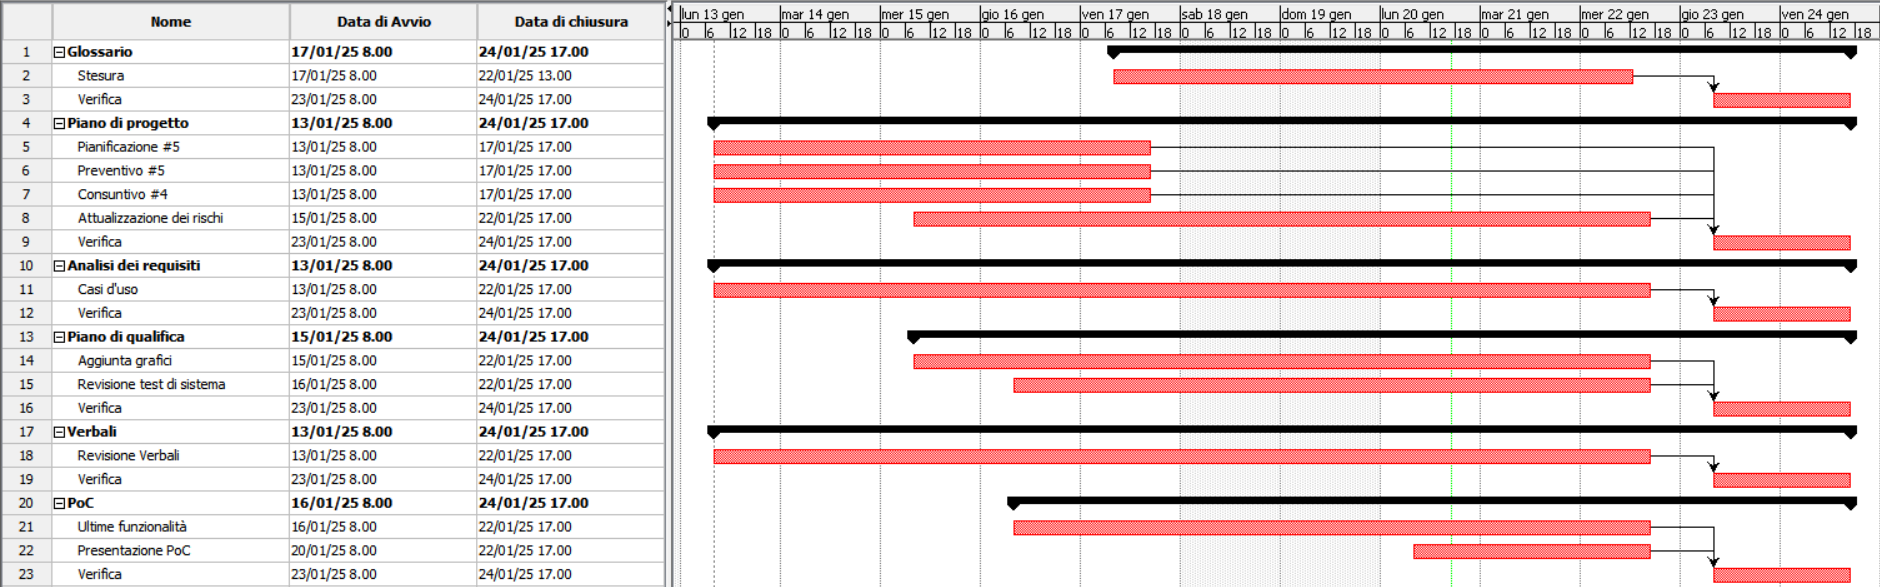
\includegraphics[scale = 0.4]{template/images/gantt5.png}
    \caption{Diagramma di Gantt sprint 5}
    \label{fig:3.5} % Etichetta per il riferimento
\end{figure}
\newpage

\subsubsection{Sprint 6 (dal 27/01/2025 al 07/02/2025)}
In questo sprint, il team si concentrerà sull'approvazione della documentazione
relativa alla RTB. Come passo preliminare, verranno aggiunti i termini mancanti
al documento \textit{Glossario} e verranno eseguite piccole modifiche al
documento \textit{Analisi dei requisiti}. Successivamente, sarà organizzato un
incontro con il professor Cardin Riccardo per presentare il PoC e completare la
prima fase di revisione della RTB. La durata dello sprint sarà quella standard,
sebbene il numero di attività sia inferiore a causa degli impegni di studio dei
membri del team.

\begin{figure}[h!]
    \centering
    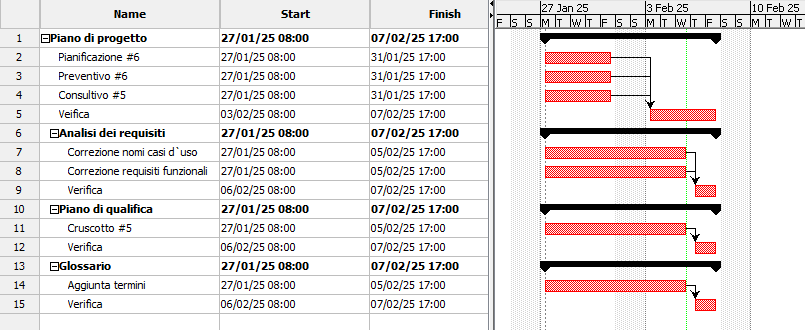
\includegraphics[scale = 0.6]{template/images/gantt6.png}
    \caption{Diagramma di Gantt sprint 6}
    \label{fig:3.6} % Etichetta per il riferimento
\end{figure}

\subsubsection{Sprint 7 (dal 10/02/2025 al 21/02/2025)}
Il settimo sprint sarà dedicato all'integrazione delle tecnologie necessarie
per lo sviluppo del progetto. In particolare, verrà aggiunto il backend al PoC,
che sarà quindi completato; conseguentemente, verrà integrata la lista dei
requisiti di vincolo. Quindi chiederemo un secondo incontro con il professor
Cardin Riccardo per presentare quanto fatto e ricevere un feedback.\\ Inoltre,
verrà redatto il resoconto delle attività di verifica nel \textit{Piano di
qualifica}, relativamente agli sprint 5 e 6. Oltre al \textit{Verbale interno} 
di fine sprint, verrà redatto anche il \textit{Verbale esterno} dell'incontro
del 22-01-2025. Infine, verrà aggiornato il \textit{Glossario} con i nuovi termini introdotti.
\begin{figure}[h!]
    \centering
    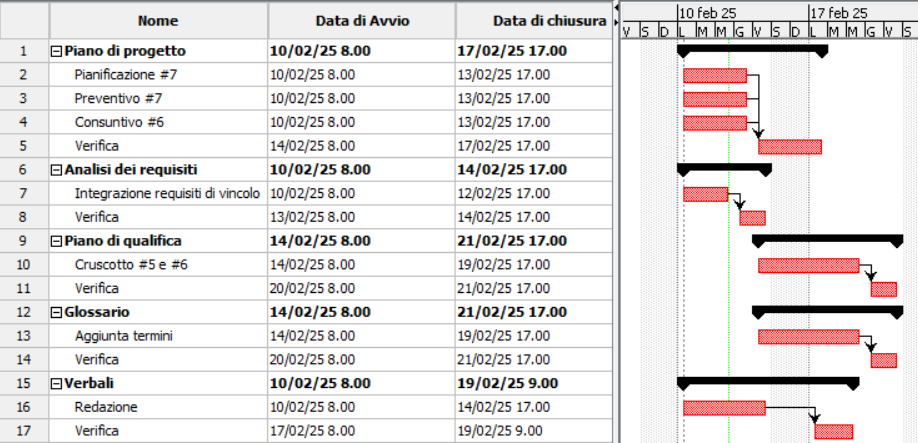
\includegraphics[scale = 0.65]{template/images/gantt7.png}
    \caption{Diagramma di Gantt sprint 7}
    \label{fig:3.7} % Etichetta per il riferimento
\end{figure}
\newpage

\subsubsection{Sprint 8 (dal 24/02/2025 al 27/02/2025)}
Durante l'ottavo sprint, ci dedicheremo al perfezionamento dell'organizzazione del repository e all'ottimizzazione della GitHub Page.
Affronteremo anche le eventuali modifiche all'\textit{Analisi dei requisiti} suggerite dal professor Riccardo Cardin.
Inoltre, è in programma un incontro con il proponente per un approfondimento sulle prestazioni del software e sulle soluzioni tecniche adottate.
Data la ridotta mole di lavoro restante per la presentazione dell'RTB, questo sprint avrà una durata di una sola settimana.

\begin{figure}[h!]
    \centering
    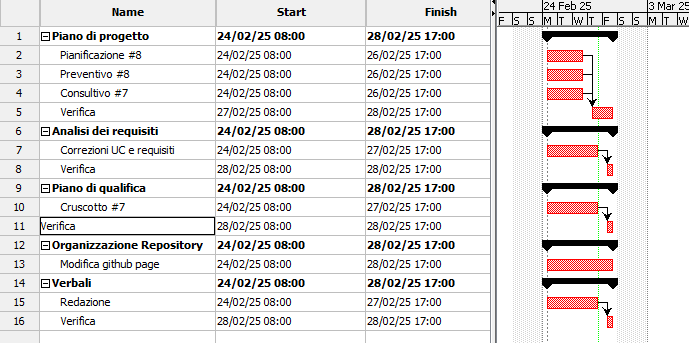
\includegraphics[scale = 0.7]{template/images/gantt8.png}
    \caption{Diagramma di Gantt sprint 8}
    \label{fig:3.8} % Etichetta per il riferimento
\end{figure}


\pagebreak

\section{Preventivo}
In questa sezione viene pianificata nel dettaglio la suddivisione dei ruoli con
le corrispondenti ore di lavoro per ogni componente del gruppo e viene fornito
un preventivo, sia relativamente all'intera durata del progetto, sia
relativamente ad ogni periodo di lavoro.

\subsection{Ore totali}
Il team ha deciso di suddividere le ore individuali in modo equivalente,
assegnando un totale di 92 ore a ciascun membro. Di seguito si riporta la
distribuzione delle ore per ruolo e il calcolo dei costi totali.


\newcommand{\costTable}[1]{

\renewcommand{\arraystretch}{1.5}
\rowcolors{2}{pari}{dispari}
\begin{longtable}{ %0.87
		>{\centering}M{0.20\textwidth} 
		>{\centering}M{0.10\textwidth}
		>{\centering}M{0.10\textwidth}
		>{\centering}M{0.10\textwidth} 
		>{\centering\arraybackslash}M{0.15\textwidth} 
		 }
	\rowcolorhead
	\headertitle{} &
	\centering \headertitle{Ore ind.} &	
	\headertitle{Ore tot.} &
	\headertitle{Costo (\euro/h)} & 
	\headertitle{Costo Totale (\euro)} 
	\endfirsthead	
	\endhead
	
	#1

\end{longtable}
\vspace{1em}

}
\costTable{
    Responsabile& 9 & 54 & 30 &  1620\tabularnewline
    Amministratore& 7 & 42 & 20 &  840\tabularnewline
    Analista& 16 & 96 & 25 &  2400\tabularnewline
	Progettista& 20 & 120 & 25 &  3000\tabularnewline
	Programmatore & 22 & 132 & 15 &  1980 \\
	Verificatore& 18 & 108 & 15 &  1620\tabularnewline
 \midrule[\heavyrulewidth] 
 \textbf{TOTALE}& 92 & 552 & - &  11460\tabularnewline
}

\subsection{Costo Totale}
Il costo finale calcolato in base alle tariffe orarie dei ruoli e alle ore
preventivate risulta di: \textbf{\euro 11460}.
\pagebreak
\subsection{RTB}
\subsubsection{Sprint 1}
Per il primo sprint, i ruoli necessari per raggiungere gli obiettivi
pianificati sono:
\begin{itemize}
    \item Responsabile;
    \item Amministratore;
    \item Verificatore;
    \item Analista.
\end{itemize}

Di seguito una tabella dettagliata con la distribuzione dei ruoli e delle ore previsti per ciascun membro.


\newcommand{\memberTable}[1]{

	\renewcommand{\arraystretch}{1.5}
	\rowcolors{2}{pari}{dispari}
	\begin{longtable}{ %0.87
		>{\centering}M{0.22\textwidth}
		>{\centering}M{0.08\textwidth}
		>{\centering}M{0.08\textwidth}
		>{\centering}M{0.08\textwidth}
		>{\centering}M{0.08\textwidth}
		>{\centering}M{0.08\textwidth}
		>{\centering}M{0.08\textwidth}
		>{\centering\arraybackslash}M{0.08\textwidth}
		}
		\rowcolorhead
		\headertitle{Membro} &
		\headertitle{Resp.}  &
		\headertitle{Amm.}   &
		\headertitle{An.}    &
		\headertitle{Proge.} &
		\headertitle{Progr.} &
		\headertitle{Ver.}   &
		\headertitle{TOT.}
		\endfirsthead
		\endhead

		#1

	\end{longtable}
	\vspace{1em}

}

\memberTable{
    Bergamin Elia & 5 & - & - & - & - & - & \textbf{5}\tabularnewline
    Diviesti Filippo & - & - & - & - & - & 6 & \textbf{6}\tabularnewline
    Djossa Edgar & - & 5 & - & - & - & - & \textbf{5}\tabularnewline
    Chilese Elena & - & - & 7 & - & - & - & \textbf{7}\tabularnewline
    Pincin Matteo & - & - & - & - & - & 6 & \textbf{6}\tabularnewline
    Soranzo Andrea & - & 5 & - & - & - & - & \textbf{5}\tabularnewline
    \midrule[\heavyrulewidth]
    \textbf{TOTALE}& 5 & 10 & 7 & - & - & 12 & \textbf{34}\tabularnewline

    \rowcolor{white}\caption{Distribuzione delle ore preventivate per lo sprint 1}

}


I costi stimati per il primo sprint sono riportati nella tabella seguente:


\newcommand{\costTable}[1]{

	\renewcommand{\arraystretch}{1.5}
	\rowcolors{2}{pari}{dispari}
	\begin{longtable}{ %0.87
		>{\centering}M{0.20\textwidth}
		>{\centering}M{0.10\textwidth}
		>{\centering}M{0.10\textwidth}
		>{\centering}M{0.10\textwidth}
		>{\centering\arraybackslash}M{0.15\textwidth}
		}
		\rowcolorhead
		\headertitle{Ruolo}            &
		\centering
		\headertitle{Ore}              &
		\headertitle{Costo  (\euro/h)} &
		\headertitle{Costo Totale (\euro)}
		\endfirsthead
		\endhead

		#1

	\end{longtable}
	\vspace{1em}

}

\costTable{
    Responsabile & 5 & 30 & 150 \tabularnewline
    Amministratore & 10 & 20 & 200 \tabularnewline
    Analista & 7 & 25 & 175 \tabularnewline
    Progettista & - & 25 & - \tabularnewline
    Programmatore & - & 15 & - \tabularnewline
    Verificatore & 12 & 15 & 180 \tabularnewline
    \midrule[\heavyrulewidth]
    \textbf{TOTALE} & 34 & - & 705 \tabularnewline

    \rowcolor{white}\caption{Preventivo costi sprint 1}

}


\pagebreak 
\subsubsection{Sprint 2}
Per il secondo sprint, i ruoli necessari per raggiungere gli obiettivi
pianificati sono:
\begin{itemize}
    \item Responsabile;
    \item Amministratore;
    \item Verificatore;
    \item Analista.
\end{itemize}


Di seguito una tabella dettagliata con la distribuzione dei ruoli e delle ore previsti per ciascun membro.


\memberTable{
    Bergamin Elia & - & - & - & - & - & 7 & \textbf{7}\tabularnewline
    Diviesti Filippo & - & - & 9 & - & - & - & \textbf{9}\tabularnewline
    Djossa Edgar & 5 & - & - & - & - & - & \textbf{5}\tabularnewline
    Chilese Elena & - & 7 & - & - & - & - & \textbf{7}\tabularnewline
    Pincin Matteo & - & - & 9 & - & - & - & \textbf{9}\tabularnewline
    Soranzo Andrea & - & - & - & - & - & 7 & \textbf{7}\tabularnewline
    \midrule[\heavyrulewidth]
    \textbf{TOTALE}& 5 & 7 & 18 & - & - & 14 & \textbf{44}\tabularnewline

    \rowcolor{white}\caption{Distribuzione delle ore preventivate per lo sprint 2}

}


I costi stimati per il secondo sprint sono riportati nella tabella seguente:


\costTable{
    Responsabile & 5 & 30 & 150 \tabularnewline
    Amministratore & 7 & 20 & 140 \tabularnewline
    Analista & 18 & 25 & 450 \tabularnewline
    Progettista & - & 25 & - \tabularnewline
    Programmatore & - & 15 & - \tabularnewline
    Verificatore & 14 & 15 & 210 \tabularnewline
    \midrule[\heavyrulewidth]
    \textbf{TOTALE} & 44 & - & 950 \tabularnewline

    \rowcolor{white}\caption{Preventivo costi sprint 2}

}


\pagebreak 
\subsubsection{Sprint 3}
Per il terzo sprint, i ruoli necessari per raggiungere gli obiettivi
pianificati sono:
\begin{itemize}
    \item Responsabile;
    \item Amministratore;
    \item Verificatore;
    \item Analista.
\end{itemize}


Di seguito una tabella dettagliata con la distribuzione dei ruoli e delle ore previste per ciascun membro.


\memberTable{
    Bergamin Elia & - & 1 & 8 & - & - & - & \textbf{9}\tabularnewline
    Diviesti Filippo & 3 & - & - & - & - & - & \textbf{3}\tabularnewline
    Djossa Edgar & - & - & - & - & - & 3 & \textbf{3}\tabularnewline
    Chilese Elena & - & - & - & - & - & 3 & \textbf{3}\tabularnewline
    Pincin Matteo & - & 2 & - & - & - & - & \textbf{2}\tabularnewline
    Soranzo Andrea & - & - & 7 & - & - & - & \textbf{7}\tabularnewline
    \midrule[\heavyrulewidth]
    \textbf{TOTALE}& 3 & 3 & 15 & - & - & 6 & \textbf{27}\tabularnewline

    \rowcolor{white}\caption{Distribuzione delle ore preventivate per lo sprint 3}

}


I costi stimati per il terzo sprint sono riportati nella tabella seguente:


\costTable{
    Responsabile & 3 & 30 & 90 \tabularnewline
    Amministratore & 3 & 20 & 60 \tabularnewline
    Analista & 15 & 25 & 375 \tabularnewline
    Progettista & - & 25 & - \tabularnewline
    Programmatore & - & 15 & - \tabularnewline
    Verificatore & 6 & 15 & 90 \tabularnewline
    \midrule[\heavyrulewidth]
    \textbf{TOTALE} & 27 & - & 615 \tabularnewline

    \rowcolor{white}\caption{Preventivo costi sprint 3}

}


\pagebreak 
\subsubsection{Sprint 4}
Per il quarto sprint, i ruoli necessari per raggiungere gli obiettivi
pianificati sono:
\begin{itemize}
    \item Responsabile;
    \item Amministratore;
    \item Analista;
    \item Programmatore;
    \item Verificatore.
\end{itemize}


Di seguito una tabella dettagliata con la distribuzione dei ruoli e delle ore previste per ciascun membro.


\memberTable{
    Bergamin Elia & - & - & - & - & 3 & 2.5 & \textbf{5.5}\tabularnewline
    Diviesti Filippo & - & 2 & - & - & - & - & \textbf{2}\tabularnewline
    Djossa Edgar & - & - & 2 & - & - & - & \textbf{2}\tabularnewline
    Chilese Elena & 3 & - & - & - & - & - & \textbf{3}\tabularnewline
    Pincin Matteo & - & - & - & - & 3 & - & \textbf{3}\tabularnewline
    Soranzo Andrea & - & 2 & - & - & - & 5 & \textbf{8}\tabularnewline
    \midrule[\heavyrulewidth]
    \textbf{TOTALE}& 3 & 4 & 2 & - & 6 & 7.5 & \textbf{22.5} \tabularnewline

    \rowcolor{white}\caption{Distribuzione delle ore preventivate per lo sprint 4}

}


I costi stimati per il quarto sprint sono riportati nella tabella seguente:


\costTable{
    Responsabile & 3 & 30 & 90 \tabularnewline
    Amministratore & 4 & 20 & 80 \tabularnewline
    Analista & 2 & 25 & 50 \tabularnewline
    Progettista & - & 25 & - \tabularnewline
    Programmatore & 6 & 15 & 90 \tabularnewline
    Verificatore & 7.5 & 15 & 112.5 \tabularnewline
    \midrule[\heavyrulewidth]
    \textbf{TOTALE} & 22.5 & - & 422.5 \tabularnewline

    \rowcolor{white}\caption{Preventivo costi sprint 4}

}


\pagebreak
\subsubsection{Sprint 5}
Per il quinto sprint, i ruoli necessari per raggiungere gli obiettivi
pianificati sono:
\begin{itemize}
    \item Responsabile;
    \item Amministratore;
    \item Analista;
    \item Programmatore;
    \item Verificatore.
\end{itemize}


Di seguito una tabella dettagliata con la distribuzione dei ruoli e delle ore previste per ciascun membro.


\memberTable{
    Bergamin Elia & - & 2 & - & - & - & 3 & \textbf{5}\tabularnewline
    Diviesti Filippo & - & - & - & - & - & 4 & \textbf{4}\tabularnewline
    Djossa Edgar & - & - & 2 & - & 2 & - & \textbf{4}\tabularnewline
    Chilese Elena & - & - & 2 & - & - & 3 & \textbf{5}\tabularnewline
    Pincin Matteo & 6 & - & - & - & - & - & \textbf{6}\tabularnewline
    Soranzo Andrea & - & - & 6 & - & - & - & \textbf{6}\tabularnewline
    \midrule[\heavyrulewidth]
    \textbf{TOTALE}& 6 & 2 & 10 & - & 2 & 10 & \textbf{30} \tabularnewline

    \rowcolor{white}\caption{Distribuzione delle ore preventivate per lo sprint 5}

}


I costi stimati per il quinto sprint sono riportati nella tabella seguente:


\costTable{
    Responsabile & 6 & 30 & 180 \tabularnewline
    Amministratore & 2 & 20 & 40 \tabularnewline
    Analista & 10 & 25 & 250 \tabularnewline
    Progettista & - & 25 & - \tabularnewline
    Programmatore & 2 & 15 & 30 \tabularnewline
    Verificatore & 10 & 15 & 150 \tabularnewline
    \midrule[\heavyrulewidth]
    \textbf{TOTALE} & 30 & - & 650 \tabularnewline

    \rowcolor{white}\caption{Preventivo costi sprint 5}

}


\pagebreak 
\subsubsection{Sprint 6}
Per il sesto sprint, i ruoli necessari per raggiungere gli obiettivi
pianificati sono:
\begin{itemize}
    \item Responsabile;
    \item Amministratore;
    \item Analista;
    \item Verificatore.
\end{itemize}


Di seguito una tabella dettagliata con la distribuzione dei ruoli e delle ore previste per ciascun membro.


\memberTable{
    Bergamin Elia & - & - & - & - & - & 2 & \textbf{2}\tabularnewline
    Diviesti Filippo & - & 1 & - & - & - & - & \textbf{1}\tabularnewline
    Djossa Edgar & - & - & 1 & - & - & - & \textbf{1}\tabularnewline
    Chilese Elena & - & - & 2 & - & - & - & \textbf{2}\tabularnewline
    Pincin Matteo & - & - & - & - & - & 2 & \textbf{2}\tabularnewline
    Soranzo Andrea & 2 & - & - & - & - & - & \textbf{2}\tabularnewline
    \midrule[\heavyrulewidth]
    \textbf{TOTALE}& 2 & 1 & 3 & - & - & 4 & \textbf{10} \tabularnewline

    \rowcolor{white}\caption{Distribuzione delle ore preventivate per lo sprint 6}

}


I costi stimati per il sesto sprint sono riportati nella tabella seguente:


\costTable{
    Responsabile & 2 & 30 & 60 \tabularnewline
    Amministratore & 1 & 20 & 20 \tabularnewline
    Analista & 3 & 25 & 75 \tabularnewline
    Progettista & - & 25 & - \tabularnewline
    Programmatore & - & 15 & - \tabularnewline
    Verificatore & 4 & 15 & 60 \tabularnewline
    \midrule[\heavyrulewidth]
    \textbf{TOTALE} & 10 & - & 215 \tabularnewline

    \rowcolor{white}\caption{Preventivo costi sprint 6}

}

\pagebreak 
\subsubsection{Sprint 7}

Per il settimo sprint, i ruoli necessari per raggiungere gli obiettivi
pianificati sono:
\begin{itemize}
    \item Responsabile;
    \item Amministratore;
    \item Analista;
    \item Programmatore;
    \item Verificatore.
\end{itemize}


Di seguito una tabella dettagliata con la distribuzione dei ruoli e delle ore previste per ciascun membro.


\memberTable{
    Bergamin Elia & 2 & - & - & - & - & - & \textbf{2}\tabularnewline
    Diviesti Filippo & - & - & - & - & - & 1 & \textbf{1}\tabularnewline
    Djossa Edgar & - & 2 & - & - & - & - & \textbf{2}\tabularnewline
    Chilese Elena & - & - & - & - & - & 1 & \textbf{1}\tabularnewline
    Pincin Matteo & - & - & 3 & - & - & - & \textbf{3}\tabularnewline
    Soranzo Andrea & - & - & - & - & 2 & - & \textbf{2}\tabularnewline
    \midrule[\heavyrulewidth]
    \textbf{TOTALE}& 2 & 2 & 3 & - & 2 & 2 & \textbf{11} \tabularnewline

    \rowcolor{white}\caption{Distribuzione delle ore preventivate per lo sprint 7}

}


I costi stimati per il settimo sprint sono riportati nella tabella seguente:


\costTable{
    Responsabile & 2 & 30 & 60 \tabularnewline
    Amministratore & 2 & 20 & 40 \tabularnewline
    Analista & 3 & 25 & 75 \tabularnewline
    Progettista & - & 25 & - \tabularnewline
    Programmatore & 2 & 15 & 30 \tabularnewline
    Verificatore & 2 & 15 & 30 \tabularnewline
    \midrule[\heavyrulewidth]
    \textbf{TOTALE} & 11 & - & 235 \tabularnewline

    \rowcolor{white}\caption{Preventivo costi sprint 7}

}


\pagebreak 
\subsubsection{Sprint 8}

Per l'ottavo sprint, i ruoli necessari per raggiungere gli obiettivi
pianificati sono:
\begin{itemize}
    \item Responsabile;
    \item Amministratore;
    \item Analista;
    \item Verificatore.
\end{itemize}


Di seguito una tabella dettagliata con la distribuzione dei ruoli e delle ore previste per ciascun membro.


\memberTable{
    Bergamin Elia & - & - & - & - & - & 1 & \textbf{1}\tabularnewline
    Diviesti Filippo & - & 1 & - & - & - & - & \textbf{1}\tabularnewline
    Djossa Edgar & - & - & - & - & - & 1 & \textbf{1}\tabularnewline
    Chilese Elena & - & - & 3 & - & - & - & \textbf{3}\tabularnewline
    Pincin Matteo & - & 1 & - & - & - & - & \textbf{1}\tabularnewline
    Soranzo Andrea & 3.5 & - & - & - & - & - & \textbf{3.5}\tabularnewline
    \midrule[\heavyrulewidth]
    \textbf{TOTALE}& 3.5 & 2 & 3 & - & - & 2 & \textbf{10.5} \tabularnewline

    \rowcolor{white}\caption{Distribuzione delle ore preventivate per lo sprint 8}

}


I costi stimati per l'ottavo sprint sono riportati nella tabella seguente:


\costTable{
    Responsabile & 3.5 & 30 & 105 \tabularnewline
    Amministratore & 2 & 20 & 40 \tabularnewline
    Analista & 3 & 25 & 75 \tabularnewline
    Progettista & - & 25 & - \tabularnewline
    Programmatore & - & 15 & - \tabularnewline
    Verificatore & 2 & 15 & 30 \tabularnewline
    \midrule[\heavyrulewidth]
    \textbf{TOTALE} & 10.5 & - & 250 \tabularnewline

    \rowcolor{white}\caption{Preventivo costi sprint 8}

}

\pagebreak

\section{Consuntivo}
\subsection{Introduzione}
Questa sezione riporta i dati raccolti durante il progetto riguardo alla
ripartizione dei ruoli e alle ore impiegate da ogni componente del gruppo. Tali
dati sono comparati alle previsioni presenti nella sezione di preventivo.

\subsection{RTB}

\subsubsection{Sprint 1}
Di seguito la suddivisione dei ruoli e le ore di lavoro effettive impiegate in
questo sprint:


\newcommand{\memberReportTable}[1]{

	\renewcommand{\arraystretch}{1.5}
	\rowcolors{2}{pari}{dispari}
	\begin{longtable}{ %0.87
		>{\centering}M{0.22\textwidth}
		>{\centering}M{0.08\textwidth}
		>{\centering}M{0.08\textwidth}
		>{\centering}M{0.08\textwidth}
		>{\centering}M{0.08\textwidth}
		>{\centering}M{0.08\textwidth}
		>{\centering}M{0.08\textwidth}
		>{\centering\arraybackslash}M{0.08\textwidth}
		}
		\rowcolorhead
		\headertitle{Membro} &
		\headertitle{Resp.}  &
		\headertitle{Amm.}   &
		\headertitle{An.}    &
		\headertitle{Proge.} &
		\headertitle{Progr.} &
		\headertitle{Ver.}   &
		\headertitle{TOT.}
		\endfirsthead
		\endhead

		#1

	\end{longtable}
	\vspace{1em}

}

\memberReportTable{
    Bergamin Elia       & 5 & - & - & - & - & - & \textbf{5}\tabularnewline
    Diviesti Filippo    & - & - & - & - & - & 6 & \textbf{6}\tabularnewline
    Djossa Edgar        & - & 5 & - & - & - & - & \textbf{5}\tabularnewline
    Chilese Elena       & - & - & 3 (-4) & - & - & - & \textbf{3 (-4)}\tabularnewline
    Pincin Matteo       & - & - & - & - & - & 6 & \textbf{6}\tabularnewline
    Soranzo Andrea      & - & 5 & - & - & - & - & \textbf{5}\tabularnewline
    \midrule[\heavyrulewidth]
    \textbf{TOTALE}     & 5 & 10 & 3 (-4) & - & - & 12 & \textbf{30 (-4)}\tabularnewline

    \rowcolor{white}\caption{Rendiconto effettivo della distribuzione delle ore per lo sprint 1}

}


I costi effettivi del periodo sono i seguenti:


\newcommand{\costReportTable}[1]{

	\renewcommand{\arraystretch}{1.5}
	\rowcolors{2}{pari}{dispari}
	\begin{longtable}{ %0.87
		>{\centering}M{0.30\textwidth}
		>{\centering}M{0.10\textwidth}
		>{\centering}M{0.10\textwidth}
		>{\centering}M{0.10\textwidth}
		>{\centering\arraybackslash}M{0.15\textwidth}
		}
		\rowcolorhead
		\headertitle{Ruolo}            &
		\centering
		\headertitle{Ore}              &
		\headertitle{Costo  (\euro/h)} &
		\headertitle{Costo Totale (\euro)}
		\endfirsthead
		\endhead

		#1

	\end{longtable}
	\vspace{1em}

}

\costReportTable{
    Responsabile & 5 & 30 & 150 \tabularnewline
    Amministratore & 10 & 20 & 200 \tabularnewline
    Analista & 3 (-4) & 25 & 75 (-100) \tabularnewline
    Progettista & - & 25 & - \tabularnewline
    Programmatore & - & 15 & - \tabularnewline
    Verificatore & 12 & 15 & 180 \tabularnewline
    \midrule[\heavyrulewidth]
    \textbf{Totale Consuntivo} & 30 & - & 605 \tabularnewline
    \midrule[\heavyrulewidth]
    \textbf{Totale Preventivo} & 34 & - & 705 \tabularnewline
    \midrule[\heavyrulewidth]
    \textbf{Differenza} & -4 & - & -100 \tabularnewline

    \rowcolor{white}\caption{Consuntivo costi sprint 1}

}


\subsubsubsection{Resoconto}
Nel seguente resoconto vengono analizzate le principali differenze tra le stime iniziali e le ore effettive durante lo sprint:
\begin{itemize}
    \item \textbf{Analista (-4 ore):} Alla fine sono state necessarie meno ore di lavoro da parte
          dell'Analista rispetto al previsto. Questa variazione è legata, oltre che alla nostra inesperienza nel calcolo
          accurato dei tempi necessari, principalmente ad impegni di altre materie universitarie.

\end{itemize}
Nel complesso, il lavoro svolto durante lo sprint è stato in linea con gli obiettivi prefissati, sebbene siano emerse alcune differenze rispetto alle stime iniziali.\\
Per gli sprint successivi, sarà necessario affinare la fase di preventivazione, valutando con
maggiore precisione la complessità delle attività, così da ottenere stime ancora più accurate.\\

Di seguito le ore rimanenti ad ogni componente del gruppo relative ad ogni
ruolo. 
\newcommand{\remainingHoursTable}[1]{

	\renewcommand{\arraystretch}{1.5}
	\rowcolors{2}{pari}{dispari}
	\begin{longtable}{ %0.87
		>{\centering}M{0.22\textwidth}
		>{\centering}M{0.08\textwidth}
		>{\centering}M{0.08\textwidth}
		>{\centering}M{0.08\textwidth}
		>{\centering}M{0.08\textwidth}
		>{\centering}M{0.08\textwidth}
		>{\centering}M{0.08\textwidth}
		>{\centering\arraybackslash}M{0.08\textwidth}
		}
		\rowcolorhead
		\headertitle{Membro} &
		\headertitle{Resp.}  &
		\headertitle{Amm.}   &
		\headertitle{An.}    &
		\headertitle{Proge.} &
		\headertitle{Progr.} &
		\headertitle{Ver.}   
		\endfirsthead
		\endhead

		#1

	\end{longtable}
	\vspace{1em}

}
\remainingHoursTable{
    Bergamin Elia & 4 & 7 & 16 & 20 & 22 & 18 \tabularnewline
    Diviesti Filippo & 9 & 7 & 16 & 20 & 22 & 12 \tabularnewline
    Djossa Edgar & 9 & 2 & 16 & 20 & 22 & 18 \tabularnewline
    Chilese Elena & 9 & 7 & 13 & 20 & 22 & 18 \tabularnewline
    Pincin Matteo & 9 & 7 & 16 & 20 & 22 & 12 \tabularnewline
    Soranzo Andrea & 9 & 2 & 16 & 20 & 22 & 18\tabularnewline
    
    \rowcolor{white}\caption{Ore rimanenti per ogni ruolo dopo lo Sprint 1}
}

\pagebreak
\subsubsection{Sprint 2}
Di seguito la suddivisione dei ruoli e le ore di lavoro effettive impiegate in
questo sprint:


\memberReportTable{
    Bergamin Elia       & 2 (+2) & 4 (+4) & - & - & - & 5 (-2) & \textbf{11 (+4)}\tabularnewline
    Diviesti Filippo    & - & - & 9 & - & - & - & \textbf{9}\tabularnewline
    Djossa Edgar        & 5 & - & - & - & - & - & \textbf{5}\tabularnewline
    Chilese Elena       & - & 7 & - & - & - & - & \textbf{7}\tabularnewline
    Pincin Matteo       & - & - & 9 & - & - & - & \textbf{9}\tabularnewline
    Soranzo Andrea      & - & 1 (+1) & - & - & - & 7 & \textbf{8 (+1)}\tabularnewline
    \midrule[\heavyrulewidth]
    \textbf{TOTALE}     & 7 (+2) & 12 (+5) & 18 & - & - & 12 (-2) & \textbf{49 (+5)}\tabularnewline

    \rowcolor{white}\caption{Rendiconto effettivo della distribuzione delle ore per lo sprint 2}

}


I costi effettivi del periodo sono i seguenti:


\costReportTable{
    Responsabile & 7 (+2) & 30 & 210 (+60) \tabularnewline
    Amministratore & 12 (+5) & 20 & 240 (+100) \tabularnewline
    Analista & 18 & 25 & 450 \tabularnewline
    Progettista & - & 25 & - \tabularnewline
    Programmatore & - & 15 & - \tabularnewline
    Verificatore & 12 (-2) & 15 & 180 (-30) \tabularnewline
    \midrule[\heavyrulewidth]
    \textbf{Totale Consuntivo} & 49 & - & 1080 \tabularnewline
    \midrule[\heavyrulewidth]
    \textbf{Totale Preventivo} & 44 & - & 950 \tabularnewline
    \midrule[\heavyrulewidth]
    \textbf{Differenza} & 5 & - & 130 \tabularnewline

    \rowcolor{white}\caption{Consuntivo costi sprint 2}

}


\subsubsubsection{Resoconto}
Nel seguente resoconto vengono analizzate le principali differenze tra le stime iniziali e le ore effettive durante lo sprint:
\begin{itemize}
    \item \textbf{Verificatore (-2 ore);}
    \item \textbf{Responsabile (+2 ore);}
    \item \textbf{Amministratore (+5 ore).}
\end{itemize}
Sono state eseguite meno ore da verificatore poichè l'ammontare è stato leggermente sovrastimato.
Inoltre le ore aggiuntive di responsabile e amministratore si evincono dal fatto che si ha avuto più tempo da dedicare al progetto rispetto
a quello preventivato.
\\
Nel complesso, anche grazie al lavoro aggiuntivo svolto, sono stati rispettati tutti gli obiettivi prefissati per questo sprint.\\

Di seguito le ore rimanenti ad ogni componente del gruppo relative ad ogni
ruolo. \remainingHoursTable{
    Bergamin Elia & 2 & 3 & 16 & 20 & 22 & 13 \tabularnewline
    Diviesti Filippo & 9 & 7 & 7 & 20 & 22 & 12 \tabularnewline
    Djossa Edgar & 4 & 2 & 16 & 20 & 22 & 18 \tabularnewline
    Chilese Elena & 9 & 0 & 13 & 20 & 22 & 18 \tabularnewline
    Pincin Matteo & 9 & 7 & 7 & 20 & 22 & 12 \tabularnewline
    Soranzo Andrea & 9 & 1 & 16 & 20 & 22 & 11\tabularnewline
    
    \rowcolor{white}\caption{Ore rimanenti per ogni ruolo dopo lo Sprint 2}
}

\pagebreak
\subsubsection{Sprint 3}
Di seguito la suddivisione dei ruoli e le ore di lavoro effettive impiegate in
questo sprint:


\memberReportTable{
    Bergamin Elia       & - & 1 & 5 (-3) & - & - & - & \textbf{6 (-3)}\tabularnewline
    Diviesti Filippo    & 4 (+1) & - & - & - & - & - & \textbf{4 (+1)}\tabularnewline
    Djossa Edgar        & - & 0.5 (+0.5) & - & - & - & 5 (+2) & \textbf{5.5 (+2.5)}\tabularnewline
    Chilese Elena       & - & - & - & - & - & 4 (+1) & \textbf{4 (+1)}\tabularnewline
    Pincin Matteo       & - & 4 (+2) & - & - & - & - & \textbf{4 (+2)}\tabularnewline
    Soranzo Andrea      & - & - & 6 (-1) & - & - & - & \textbf{6 (-1)}\tabularnewline
    \midrule[\heavyrulewidth]
    \textbf{TOTALE}     & 4 (+1) & 5.5 (+2.5) & 11 (-4) & - & - & 9 (+3) & \textbf{29.5 (+2.5)} \tabularnewline

    \rowcolor{white}\caption{Rendiconto effettivo della distribuzione delle ore per lo sprint 3}

}


I costi effettivi del periodo sono i seguenti:


\costReportTable{
    Responsabile & 4 (+1) & 30 & 120 (+30) \tabularnewline
    Amministratore & 5.5 (+2.5) & 20 & 110 (+50) \tabularnewline
    Analista & 11 (-4) & 25 & 275 (-100) \tabularnewline
    Progettista & - & 25 & - \tabularnewline
    Programmatore & - & 15 & - \tabularnewline
    Verificatore & 9 (+3) & 15 & 135 (+45) \tabularnewline
    \midrule[\heavyrulewidth]
    \textbf{Totale Consuntivo} & 29.5 & - & 640 \tabularnewline
    \midrule[\heavyrulewidth]
    \textbf{Totale Preventivo} & 27 & - & 615 \tabularnewline
    \midrule[\heavyrulewidth]
    \textbf{Differenza} & 2.5 & - & 25 \tabularnewline

    \rowcolor{white}\caption{Consuntivo costi sprint 3}

}


\subsubsubsection{Resoconto}
Nel seguente resoconto vengono analizzate le principali differenze tra le stime iniziali e le ore effettive durante lo sprint:
\begin{itemize}
    \item \textbf{Responsabile (+1 ora);}
    \item \textbf{Amministratore (+2.5 ore);}
    \item \textbf{Analista (-4 ore);}
    \item \textbf{Verificatore (+3 ore).}
\end{itemize}

Sono state dedicate più ore al ruolo di responsabile e di amministratore
rispetto a quanto inizialmente previsto. Ciò è dovuto ad una maggiore
complessità nella gestione e organizzazione delle attività progettuali. Le ore
destinate al ruolo di analista sono state inferiori alle stime, in quanto
alcune attività di analisi sono risultate meno onerose del previsto e hanno
altresì aiutato il confronto con il proponente e l'incontro con il prof.
Cardin. Infine, il ruolo di verificatore ha richiesto un incremento di ore
rispetto al pianificato, in virtù di un aumento della complessità e
dell'estensione dei documenti da verificare. \\ Complessivamente, le variazioni
riscontrate non hanno compromesso il raggiungimento degli obiettivi prefissati,
permettendo il completamento di tutte le attività previste.\\ Di seguito le ore
rimanenti ad ogni componente del gruppo relative ad ogni ruolo.
\remainingHoursTable{
    Bergamin Elia & 2 & 2 & 11 & 20 & 22 & 13 \tabularnewline
    Diviesti Filippo & 5 & 7 & 7 & 20 & 22 & 12 \tabularnewline
    Djossa Edgar & 4 & 1.5 & 16 & 20 & 22 & 13 \tabularnewline
    Chilese Elena & 9 & 0 & 13 & 20 & 22 & 14 \tabularnewline
    Pincin Matteo & 9 & 3 & 7 & 20 & 22 & 12 \tabularnewline
    Soranzo Andrea & 9 & 1 & 10 & 20 & 22 & 11\tabularnewline
    
    \rowcolor{white}\caption{Ore rimanenti per ogni ruolo dopo lo Sprint 3}
}

\pagebreak
\subsubsection{Sprint 4}
Di seguito la suddivisione dei ruoli e le ore di lavoro effettive impiegate in
questo sprint:


\memberReportTable{
    Bergamin Elia       & - & - & - & - & 5 (+2) & 0 (-2.5) & \textbf{5 (-0.5)}\tabularnewline
    Diviesti Filippo    & - & 4 (+2) & - & - & - & - & \textbf{4 (+2)}\tabularnewline
    Djossa Edgar        & - & - & 3 (+1) & - & - & - & \textbf{3 (+1)}\tabularnewline
    Chilese Elena       & 3 & - & - & - & - & - & \textbf{3}\tabularnewline
    Pincin Matteo       & - & - & - & - & 3 & - & \textbf{3}\tabularnewline
    Soranzo Andrea      & - & 1 & - & - & - & 4.5 (-0.5) & \textbf{6.5 (-0.5)}\tabularnewline
    \midrule[\heavyrulewidth]
    \textbf{TOTALE}     & 3 & 5 (+2) & 3 (+1) & - & 8 (+2) & 4.5 (-3) & \textbf{24.5 (+2)} \tabularnewline

    \rowcolor{white}\caption{Rendiconto effettivo della distribuzione delle ore per lo sprint 4}

}


I costi effettivi del periodo sono i seguenti:


\costReportTable{
    Responsabile & 3 & 30 & 90 \tabularnewline
    Amministratore & 6 (+2) & 20 & 120 (+40) \tabularnewline
    Analista & 3 (+1) & 25 & 75 (+25) \tabularnewline
    Progettista & - & 25 & - \tabularnewline
    Programmatore & 8 (+2) & 15 & 120 (+30) \tabularnewline
    Verificatore & 4.5 (-3) & 15 & 67.5 (-45) \tabularnewline
    \midrule[\heavyrulewidth]
    \textbf{Totale Consuntivo} & 24.5 & - & 472.5 \tabularnewline
    \midrule[\heavyrulewidth]
    \textbf{Totale Preventivo} & 22.5 & - & 422.5 \tabularnewline
    \midrule[\heavyrulewidth]
    \textbf{Differenza} & 2 & - & 50 \tabularnewline

    \rowcolor{white}\caption{Consuntivo costi sprint 4}

}


\subsubsubsection{Resoconto}
Nel seguente resoconto vengono analizzate le principali differenze tra le stime iniziali e le ore effettive durante lo sprint:
\begin{itemize}
    \item \textbf{Amministratore (+2)}: la redazione dei verbali ha richiesto più tempo del solito, poiché sono stati trattati più temi nell'incontro interno e si è svolto un incontro con il proponente;
    \item \textbf{Analista (+1)}: richiesto più tempo rispetto al preventivo in quanto l'\textit{Analisi dei requisiti} conteneva più imprecisioni del previsto;
    \item \textbf{Programmatore (+2)}: lo sviluppo del PoC si è rivelato più ostico del previsto e sono state necessarie più ore per realizzare la corretta implementazione delle funzionalità richieste;
    \item \textbf{Verificatore (-3)}: lo sprint, avvenuto durante le festività natalizie, ha comportato una minore produzione di documenti rispetto al solito. Inoltre, la fase di verifica del codice del PoC è stata sovrastimata in fase di preventivo, poiché ci siamo limitati a individuare bug e imperfezioni utilizzando il PoC stesso, il che ha richiesto meno tempo.
\end{itemize}
Nonostante alcune discrepanze rispetto alle ore inizialmente stimate, tutte le attività pianificate sono state completate con successo.\\
Di seguito le ore rimanenti ad ogni componente del gruppo relative ad ogni ruolo.
\remainingHoursTable{
    Bergamin Elia & 2 & 2 & 11 & 20 & 17 & 13 \tabularnewline
    Diviesti Filippo & 5 & 3 & 7 & 20 & 22 & 12 \tabularnewline
    Djossa Edgar & 4 & 1.5 & 13 & 20 & 22 & 13 \tabularnewline
    Chilese Elena & 6 & 0 & 13 & 20 & 22 & 14 \tabularnewline
    Pincin Matteo & 9 & 3 & 7 & 20 & 19 & 12 \tabularnewline
    Soranzo Andrea & 9 & 0 & 10 & 20 & 22 & 6.5\tabularnewline
    
    \rowcolor{white}\caption{Ore rimanenti per ogni ruolo dopo lo Sprint 4}
}

\pagebreak
\subsubsection{Sprint 5}
Di seguito la suddivisione dei ruoli e le ore di lavoro effettive impiegate in
questo sprint:


\memberReportTable{
    Bergamin Elia       & - & 2 & - & - & - & 3 & \textbf{5}\tabularnewline
    Diviesti Filippo    & - & - & - & - & - & 4 & \textbf{4}\tabularnewline
    Djossa Edgar        & - & - & 2 & - & 2 & - & \textbf{4}\tabularnewline
    Chilese Elena       & - & - & 2.5 (+0.5) & - & - & 3 & \textbf{5.5 (+0.5)}\tabularnewline
    Pincin Matteo       & 5 (-1) & - & - & - & - & - & \textbf{5 (-1)}\tabularnewline
    Soranzo Andrea      & - & - & 7 (+1) & - & - & - & \textbf{7 (+1)}\tabularnewline
    \midrule[\heavyrulewidth]
    \textbf{TOTALE}     & 5 (-1) & 2 & 11.5 (+1.5) & - & 2 & 10 & \textbf{30.5 (+0.5)} \tabularnewline

    \rowcolor{white}\caption{Rendiconto effettivo della distribuzione delle ore per lo sprint 5}

}


I costi effettivi del periodo sono i seguenti:


\costReportTable{
    Responsabile & 5 (-1) & 30 & 150 (-30) \tabularnewline
    Amministratore & 2 & 20 & 40 \tabularnewline
    Analista & 11.5 (+1.5) & 25 & 287.5 (+37.5) \tabularnewline
    Progettista & - & 25 & - \tabularnewline
    Programmatore & 2 & 15 & 30 \tabularnewline
    Verificatore & 10 & 15 & 150 \tabularnewline
    \midrule[\heavyrulewidth]
    \textbf{Totale Consuntivo} & 30.5 & - & 657.5 \tabularnewline
    \midrule[\heavyrulewidth]
    \textbf{Totale Preventivo} & 30 & - & 650 \tabularnewline
    \midrule[\heavyrulewidth]
    \textbf{Differenza} & 0.5 & - & 7.5 \tabularnewline

    \rowcolor{white}\caption{Consuntivo costi sprint 5}

}


\subsubsubsection{Resoconto}
Nel seguente resoconto vengono analizzate le principali differenze tra le stime iniziali e le ore effettive durante lo sprint:
\begin{itemize}
    \item \textbf{Responsabile (-1)};
    \item \textbf{Analista (+1.5)}: La redazione e la creazione dei grafici per il cruscotto di qualità ha richiesto più tempo del previsto perché richiede azioni manuali.
\end{itemize}
In breve, oltre ad alcune difficoltà incontrate per la creazione di grafici utili a rappresentare l'andamento della qualità, tutte le attività pianificate sono state completate con successo.\\
Di seguito le ore rimanenti ad ogni componente del gruppo relative ad ogni ruolo.
\remainingHoursTable{
    Bergamin Elia & 2 & 0 & 11 & 20 & 17 & 10 \tabularnewline
    Diviesti Filippo & 5 & 3 & 7 & 20 & 22 & 8 \tabularnewline
    Djossa Edgar & 4 & 1.5 & 11 & 20 & 20 & 13 \tabularnewline
    Chilese Elena & 6 & 0 & 10.5 & 20 & 22 & 11 \tabularnewline
    Pincin Matteo & 4 & 3 & 7 & 20 & 19 & 12 \tabularnewline
    Soranzo Andrea & 9 & 0 & 3 & 20 & 22 & 6.5\tabularnewline
    
    \rowcolor{white}\caption{Ore rimanenti per ogni ruolo dopo lo Sprint 5}
}

\pagebreak
\subsubsection{Sprint 6}
Di seguito la suddivisione dei ruoli e le ore di lavoro effettive impiegate in
questo sprint:

\memberReportTable{
    Bergamin Elia       & - & - & - & - & - & 1 (-1) & \textbf{1 (-1)}\tabularnewline
    Diviesti Filippo    & - & 1 & - & - & - & - & \textbf{1}\tabularnewline
    Djossa Edgar        & - & - & 0.5 (-0.5) & - & - & - & \textbf{0.5 (-0.5)}\tabularnewline
    Chilese Elena       & - & - & 0 (-2) & - & - & - & \textbf{0 (-2)}\tabularnewline
    Pincin Matteo       & - & - & - & - & - & 0.5 (-1.5) & \textbf{0.5 (-1.5)}\tabularnewline
    Soranzo Andrea      & 2 & - & - & - & - & - & \textbf{2}\tabularnewline
    \midrule[\heavyrulewidth]
    \textbf{TOTALE}     & 2 & 1 & 0.5 (-2.5) & - & - & 1.5 (-2.5) & \textbf{5 (-5)} \tabularnewline

    \rowcolor{white}\caption{Rendiconto effettivo della distribuzione delle ore per lo sprint 6}

}


I costi effettivi del periodo sono i seguenti:

\costReportTable{
    Responsabile & 2 & 30 & 60 \tabularnewline
    Amministratore & 1 & 20 & 20 \tabularnewline
    Analista & 0.5 (-2.5) & 25 & 12.5 (-62.5) \tabularnewline
    Progettista & - & 25 & - \tabularnewline
    Programmatore & - & 15 & - \tabularnewline
    Verificatore & 1.5 (-2.5) & 15 & 22.5 (-37.5) \tabularnewline
    \midrule[\heavyrulewidth]
    \textbf{Totale Consuntivo} & 5 & - & 115 \tabularnewline
    \midrule[\heavyrulewidth]
    \textbf{Totale Preventivo} & 10 & - & 215 \tabularnewline
    \midrule[\heavyrulewidth]
    \textbf{Differenza} & -5 & - & -100 \tabularnewline

    \rowcolor{white}\caption{Consuntivo costi sprint 6}

}


\subsubsubsection{Resoconto}
Nel seguente resoconto vengono analizzate le principali differenze tra le stime iniziali e le ore effettive durante lo sprint:
\begin{itemize}
    \item \textbf{Analista (-2.5)}; 
    \item \textbf{Verificatore (-2.5)}.
\end{itemize}
Lo studio per gli esami universitari ha richiesto più tempo del previsto, riducendo le ore disponibili per il progetto.
Per questo motivo, l'analisi delle metriche di qualità è stata rinviata allo sprint successivo. 
Conseguentemente, anche le ore di verifica sono state inferiori rispetto a quanto preventivato.\\
Di seguito le ore rimanenti ad ogni componente del gruppo relative ad ogni ruolo.
\remainingHoursTable{
    Bergamin Elia & 2 & 0 & 11 & 20 & 17 & 9 \tabularnewline
    Diviesti Filippo & 5 & 2 & 7 & 20 & 22 & 8 \tabularnewline
    Djossa Edgar & 4 & 1.5 & 10.5 & 20 & 20 & 13 \tabularnewline
    Chilese Elena & 6 & 0 & 10.5 & 20 & 22 & 11 \tabularnewline
    Pincin Matteo & 4 & 3 & 7 & 20 & 19 & 11.5 \tabularnewline
    Soranzo Andrea & 7 & 0 & 3 & 20 & 22 & 6.5\tabularnewline
    
    \rowcolor{white}\caption{Ore rimanenti per ogni ruolo dopo lo Sprint 6}
}

\pagebreak
\subsubsection{Sprint 7}
Di seguito la suddivisione dei ruoli e le ore di lavoro effettive impiegate in
questo sprint:

\memberReportTable{
    Bergamin Elia       & 2 & - & - & - & - & - & \textbf{2}\tabularnewline
    Diviesti Filippo    & - & - & - & - & - & 1 & \textbf{1}\tabularnewline
    Djossa Edgar        & - & 1 (-1) & - & - & - & - & \textbf{1 (-1)}\tabularnewline
    Chilese Elena       & - & - & - & - & - & 1 & \textbf{1}\tabularnewline
    Pincin Matteo       & - & - & 2.5 (-0.5) & - & - & - & \textbf{2.5 (-0.5)}\tabularnewline
    Soranzo Andrea      & - & - & - & - & 2 & - & \textbf{2}\tabularnewline
    \midrule[\heavyrulewidth]
    \textbf{TOTALE}     & 2 & 1 (-1) & 2.5 (-0.5) & - & 2 & 2 & \textbf{9.5 (-1.5)} \tabularnewline

    \rowcolor{white}\caption{Rendiconto effettivo della distribuzione delle ore per lo sprint 7}

}


I costi effettivi del periodo sono i seguenti:

\costReportTable{
    Responsabile & 2 & 30 & 60 \tabularnewline
    Amministratore & 1 (-1) & 20 & 20 (-20) \tabularnewline
    Analista & 2.5 (-0.5) & 25 & 62.5 (-12.5) \tabularnewline
    Progettista & - & 25 & - \tabularnewline
    Programmatore & 2 & 15 & 30 \tabularnewline
    Verificatore & 2 & 15 & 30 \tabularnewline
    \midrule[\heavyrulewidth]
    \textbf{Totale Consuntivo} & 10.5 & - & 202.5 \tabularnewline
    \midrule[\heavyrulewidth]
    \textbf{Totale Preventivo} & 12 & - & 235 \tabularnewline
    \midrule[\heavyrulewidth]
    \textbf{Differenza} & -1.5 & - & -32.5 \tabularnewline

    \rowcolor{white}\caption{Consuntivo costi sprint 7}

}


\subsubsubsection{Resoconto}
Nel seguente resoconto vengono analizzate le principali differenze tra le stime iniziali e le ore effettive durante lo sprint:
\begin{itemize}
    \item \textbf{Amministratore (-1)}; 
    \item \textbf{Analista (-0.5)}.
\end{itemize}

\remainingHoursTable{
    Bergamin Elia & 0 & 0 & 11 & 20 & 17 & 9 \tabularnewline
    Diviesti Filippo & 5 & 2 & 7 & 20 & 22 & 7 \tabularnewline
    Djossa Edgar & 4 & 0.5 & 10.5 & 20 & 20 & 13 \tabularnewline
    Chilese Elena & 6 & 0 & 10.5 & 20 & 22 & 10 \tabularnewline
    Pincin Matteo & 4 & 3 & 4.5 & 20 & 19 & 11.5 \tabularnewline
    Soranzo Andrea & 7 & 0 & 3 & 20 & 20 & 6.5\tabularnewline
    
    \rowcolor{white}\caption{Ore rimanenti per ogni ruolo dopo lo Sprint 7}
}

\pagebreak

\newcommand{\riskMitigation}[1]{%
    \renewcommand{\arraystretch}{1.5}% Modifica l'altezza delle righe
    \rowcolors{2}{pari}{dispari}% Alterna i colori delle righe
    \begin{longtable}{%
        >{\centering\arraybackslash}m{0.22\textwidth}%
        >{\centering\arraybackslash}m{0.38\textwidth}%
        >{\centering\arraybackslash}m{0.38\textwidth}%
    }%
        \rowcolorhead
        \headertitle{Nome} &
        \headertitle{Descrizione} &
        \headertitle{Mitigazione} \\
        \endfirsthead
        \endhead

        #1 % Contenuto dinamico

    \end{longtable}
    \vspace{1em}
}

\section{Attualizzazione dei rischi}
In questa sezione sono riportati i rischi che si sono verificati nel corso del progetto e le relative misure di mitigazione attuate dal gruppo.

\riskMitigation{
    \textbf{Comprensione dei requisiti} & Basandosi sul capitolato, non tutti i requisiti erano chiari. & Si sono svolte delle riunioni con il proponente, per discutere e chiarire dubbi. \\
    \textbf{Inesperienza Tecnologica} & Nella fase iniziale del progetto, e durante lo sviluppo del PoC sono sorti dubbi e difficoltà rispetto all'utilizzo di GitHub e delle tecnologie proposte dall'azienda. & Ogni membro del gruppo ha ricavato del tempo personale da dedicare allo studio delle tecnologie da utilizzare, in modo da essere allineati e procedere con maggiore efficienza. \\
    \textbf{Disponibilità dei componenti} & A causa delle festività, la disponibilità dei componenti del gruppo si è ridotta durante quello sprint. & Nella pianificazione si è tenuto conto di questo fattore, inoltre, lo sprint è durato una settimana in più.\\
    \textbf{Discussioni interne} & Durante gli sprint è capitato di dover prendere delle decisioni o di avere dei dubbi, che andassero risolti prima del meeting interno di fine periodo. & È stato usato il canale di comunicazione asincrono Telegram per poter discutere e arrivare a una conclusione.
}

\pagebreak


% insert here other content (\include)


\end{document}


